% REMEMBER: You must not plagiarise anything in your report. Be extremely careful.

\documentclass{l4proj}


%
% put any additional packages here
%
\usepackage{bm}
\usepackage{booktabs}
\usepackage{graphicx}
\usepackage[export]{adjustbox}
\usepackage{newfloat}
\usepackage{float}

\DeclareFloatingEnvironment[placement={!ht},name=List]{captionedList}

\begin{document}

%==============================================================================
%% METADATA
\title{Deep neural networks for classification of multispectral images}
\author{Niklas Lindorfer}
\date{September 26, 2019}

\maketitle

%==============================================================================
%% ABSTRACT
\begin{abstract}
    Every abstract follows a similar pattern. Motivate; set aims; describe work; explain results.
    \vskip 0.5em
    ``XYZ is bad. This project investigated ABC to determine if it was better. 
    ABC used XXX and YYY to implement ZZZ. This is particularly interesting as XXX and YYY have
    never been used together. It was found that  
    ABC was 20\% better than XYZ, though it caused rabies in half of subjects.''
\end{abstract}

%==============================================================================

% EDUCATION REUSE CONSENT FORM
% If you consent to your project being shown to future students for educational purposes
% then insert your name and the date below to  sign the education use form that appears in the front of the document. 
% You must explicitly give consent if you wish to do so.
% If you sign, your project may be included in the Hall of Fame if it scores particularly highly.
%
% Please note that you are under no obligation to sign 
% this declaration, but doing so would help future students.
%
\def\consentname {Niklas Lindorfer} % your full name
\def\consentdate {26 September 2019} % the date you agree
%
\educationalconsent


%==============================================================================
\tableofcontents

%==============================================================================
%% Notes on formatting
%==============================================================================
% The first page, abstract and table of contents are numbered using Roman numerals and are not
% included in the page count. 
%
% From now on pages are numbered
% using Arabic numerals. Therefore, immediately after the first call to \chapter we need the call
% \pagenumbering{arabic} and this should be called once only in the document. 
%
% The first Chapter should then be on page 1. You are allowed 40 pages for a 40 credit project and 20 pages for a 
% 20 credit report. This includes everything numbered in Arabic numerals (excluding front matter) up
% to but excluding the appendices and bibliography.
%
% You must not alter text size (it is currently 10pt) or alter margins or spacing.
%
%
%==================================================================================================================================
%
% IMPORTANT
% The chapter headings here are **suggestions**. You don't have to follow this model if
% it doesn't fit your project. Every project should have an introduction and conclusion,
% however. 
%
%==================================================================================================================================
\chapter{Introduction}

% reset page numbering. Don't remove this!
\pagenumbering{arabic} 

%----------------------------------------------------------------------------------------------------------------------------------


\section{Motivation}

Deep convolutional neural networks have achieved impressive results on image classification tasks. The majority of image classification systems is trained on conventional visible light images. 

Thermal cameras have gotten significantly more affordable in recent years. This makes it increasingly feasible to extend computer vision systems 

%----------------------------------------------------------------------------------------------------------------------------------

\section{Aim}

The aim of this project is to explore the benefits and drawbacks of incorporating thermal imaging into an image classification model. We shall demonstrate our findings on a multi-class classification task involving eight classes of animals. To achieve this, we will:

\begin{itemize}
  \item review existing solutions for multispectral image classification systems (Section \ref{background}),
  \item analyse the problems and potential benefits involved with creating a machine learning model based on multispectral data (Section \ref{analysis}),
  \item create a dataset of eight classes of farm animals, develop strategies to prevent overfitting and implement a state-of-the-art convolutional neural network for image classification (Section \ref{design}),
  \item analyse the performance of our model compared to conventional, visible-light-only image classifiers.
\end{itemize}

%----------------------------------------------------------------------------------------------------------------------------------

\section{Potential applications}




%==================================================================================================================================
\chapter{Background}
\label{background}

\section{Imaging}
\label{imaging}

\subsection{Electromagnetic radiation}

Visible light and infrared are forms of electromagnetic radiation. Visible light (VIS) has wavelengths roughly between $400$ and $700 nm$. The hue of visible light is determined by its wavelength. Colours as perceived by human vision are the result of a spectral distribution of wavelengths of the light that enters the eye. 

Infrared light (IR), with wavelengths between $700 nm$ and $1 mm$, is generally invisible to humans. It is commonly subdivided into near infrared (NIR), short-wavelength infrared (SWIR), medium-wavelength infrared (MWIR), long-wavelength infrared (LWIR), and far infrared (FIR) \citep[p. 28]{byrnes_unexploded_2008}, as can be seen in Figure \ref{fig:em_spectrum}.

\begin{figure}[ht]
  \centering
  \begin{subfigure}[h!]{0.9\textwidth}
    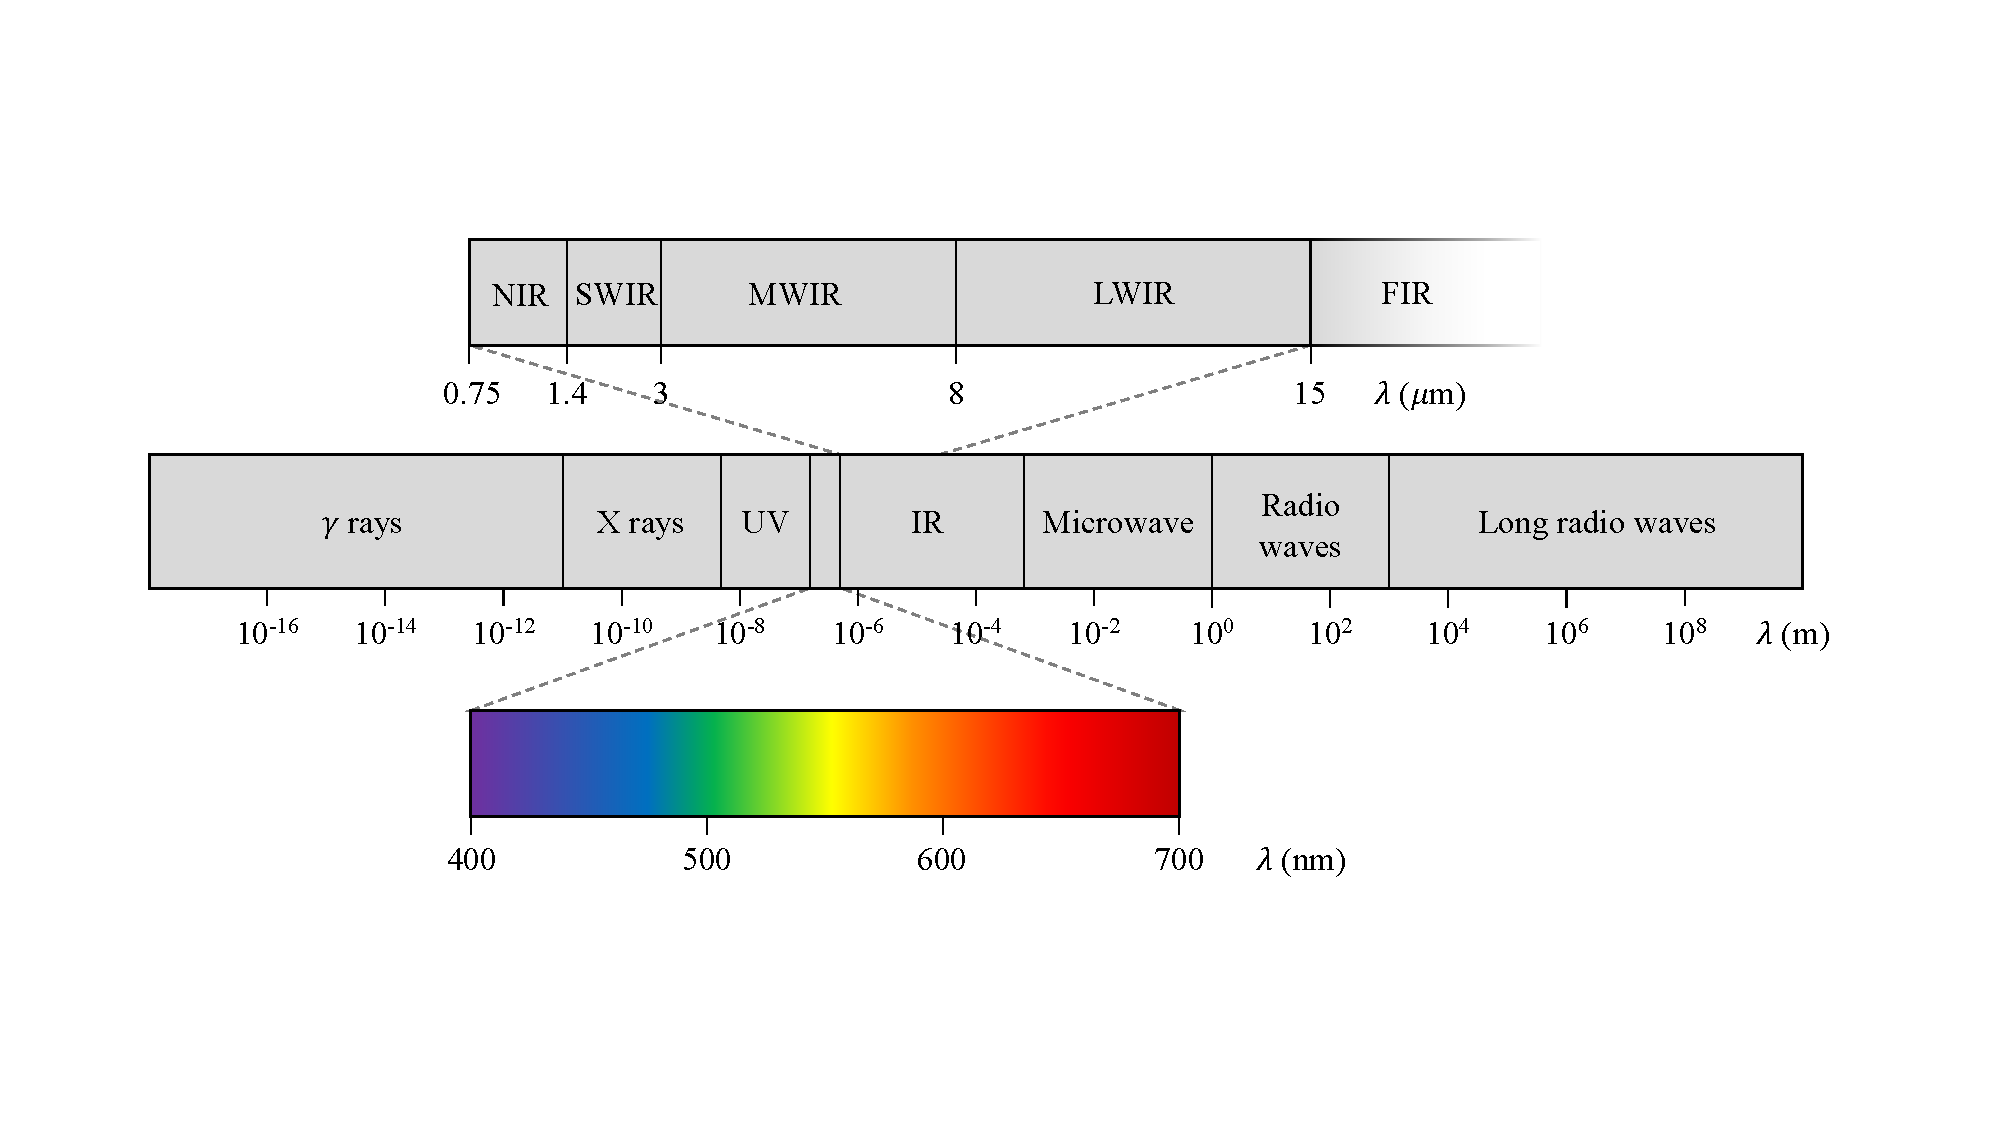
\includegraphics[width=\textwidth, trim={1.5cm 4cm 2cm 4cm}, clip=true]{images/EM_spectrum.pdf}
  \end{subfigure}
  \caption{The electromagnetic spectrum with detailled view of visible light and infrared. IR subdivisions modelled after \citet[p. 28]{byrnes_unexploded_2008}.}
  \label{fig:em_spectrum}
\end{figure}

\subsection{Thermal infrared radiation}

Black-body radiation is defined as thermal electromagnetic radiation emitted by an idealized opaque, non-reflective body \citep{young_sears_2012}. It has a continuous frequency spectrum that is dependent on the temperature of the body \citep{kogure_thermodynamic_2007}. The spectrum has a characteristic peak, which is antiproportional to the temperature $T [K]$ according to Wien's displacement law:

\begin{equation}
  \lambda_{peak} = \frac{2.898 \times 10^{-3}}{T} [m],
\end{equation}

Bodies at a room temperature of $300 K$ emit electromagnetic radiation with a peak at $9.7 \mu m$ \citep{jarc_graz_2007}, falling into the LWIR range. To account for different non-ideal surfaces, the material-specific emissivity constant $\epsilon \in [0..1]$ is introduced to describe the share of radiation that is emitted by a body compared to an ideal black body. The total energy radiated by a body per unit surface and time is expressed by the Stefan-Boltzmann law:

\begin{equation}
  W = \epsilon \sigma T^4,
\end{equation}

where $\sigma$ is a proportionality constant. Thus, if the emissivity of the body is known, this law can be applied to determine its temperature. This is the theoretical foundation for thermal imaging. In practice, the material and corresponding emissivity are often undetermined. Therefore, the received infrared radiation contains an unknown share of reflected radiation, adding noise to the measurement. This can be somewhat mitigated by estimating the value of $\epsilon$.

\subsection{Spectral imaging}

Spectral images combine spatial and spectral information in a 3-D data structure where the dimensions correspond to height, width and waveband. 
A distinction is made between hyperspectral and multispectral imaging techniques. 

If an image is acquired at many (tens or hundreds) regularly sampled wavebands, one speaks of a hyperspectral image, sometimes referred to as a hypercube. Hyperspectral images have many powerful applications, including agriculture and food quality \citep{dale_hyperspectral_2013} and medical applications \citep{lu_medical_2014}. However, capturing hyperspectral images requires advanced sensing equipment. Furthermore, hypercubes are difficult to process due to the high amount of information and therefore often require the application of computationally expensive preprocessing techniques, such as dimensionality-reduction \citep{qin_hyperspectral_2013}.

Multispectral images comprise of a few discrete wavebands. As opposed to hyperspectral images, it is usually not possible to extract a full continuous spectrum of an individual pixel from multispectral images \citep{abdul_multi-disnet_2019}.


%----------------------------------------------------------------------------------------------------------------------------------

\section{Machine learning}

\subsection{Supervised and unsupervised algorithms}

Machine learning techniques can be categorised into supervised, semi-supervised, unsupervised, and reinforcement learning \citep{burkov_hundred-page_2019}.

In supervised learning, a dataset consisting of a list of labelled features $\{(\vec{x}_i, y_i)\}^N_{i=1}$ is provided. $\vec{x_i}$ is called a feature vector. The supervised learning algorithm then attempts to fit a model $f$ on the dataset such that $\forall{\vec{x_i}}. (f(\vec{x_i}) = y_i)$. The model can then be used to predict the unknown label of a test data point. In practice, a perfect fit is not possible due to noise in the dataset. Therefore, supervised algorithms are evaluated according to a loss function measuring the difference between $f(\vec{x_i})$ and $y_i$. When fitting the model, the algorithm attempts to minimise the loss over the training data. Common choices for loss functions are mean squared error (MSE) for regression and categorical cross-entropy for classification problems.

Unsupervised learning involves a dataset of unlabeled data $\{\vec{x}_i\}^N_{i=1}$. An unsupervised learning algorithm attempts to transform each feature vector $\vec{x}_i$ into another vector to solve a practical problem, such as dimensionality reduction or outlier detection \citep{burkov_hundred-page_2019}. 
This project focuses on supervised learning.

\subsection{Regression and classification}

In supervised learning, one speaks of classification or regression, depending on whether the data labels $y_i$ are discrete classes or continous, real values.


%----------------------------------------------------------------------------------------------------------------------------------


\section{Deep learning}

Deep learning is a branch of machine learning based upon the concept of artificial neural networks (ANN). ANNs leverage the concept of artificial neurons, which are an abstract model derived from biological neurons. 

\begin{figure}[ht]
  \centering
  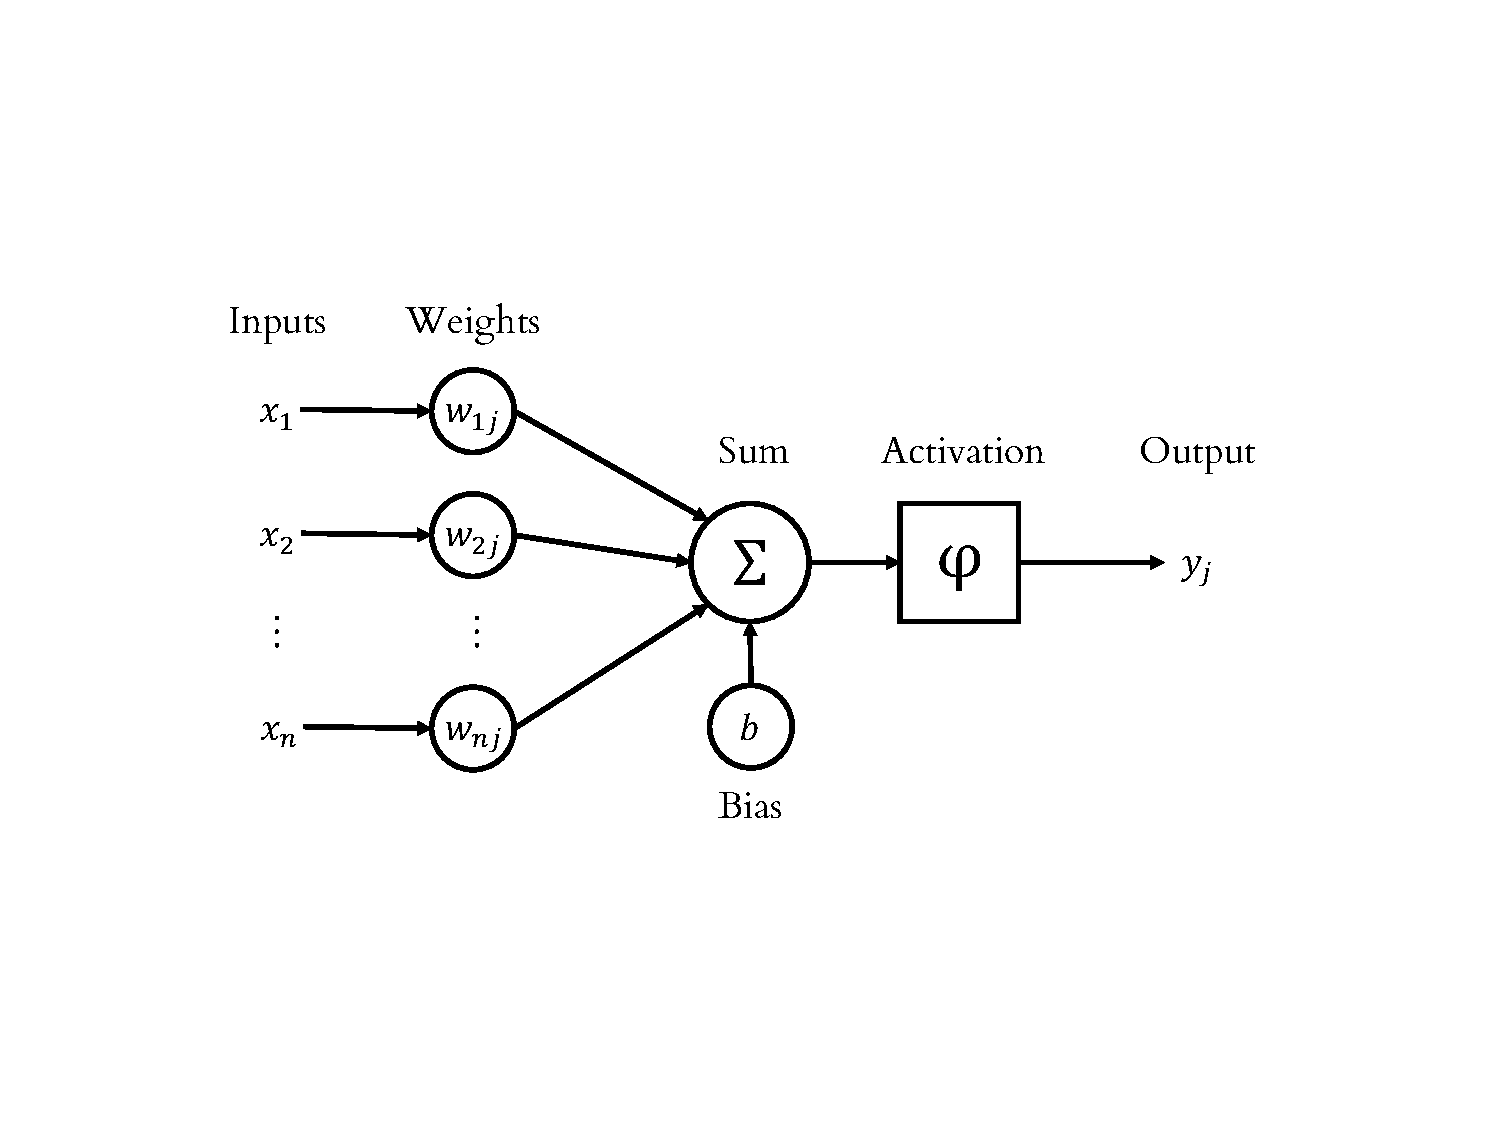
\includegraphics[width=0.5\textwidth, page={1}, trim={3.5cm 5cm 3.5cm 5cm}, clip]{images/Artificial_Neuron}
  \caption{Model of an artificial neuron.}
  \label{fig:neuron}
\end{figure}

A model of an artifical neuron is shown in Figure \ref{fig:neuron}. It consists of an input vector $\vec{x}$, a vector of weights $\vec{w}$, an optional bias $b$, an activation function $\varphi$, and an output scalar $y$. The input vector is multiplied with the weights element-wise. The sum of the result is computed and passed into the activation function, yielding the output. The output of an artificial neuron can, therefore, be computed as follows:

\begin{equation}
  y_j = \varphi (\sum_{i=0}^n x_i w_{ij}),
\end{equation}

where the bias $b$ can be treated as the first element of the input vector $\vec{x}$. A special case of the artificial neuron is the perceptron, where the activation function is a binary threshold, making the neuron output either 0 or 1 depending on the input.

In ANNs, neurons are usually grouped into fully-connected layers. For each neuron in layer $j$, $\vec{x}$ represents the outputs of all neurons of the previous layer $j-1$. A traditional feed-forward neural network thus consists of an input layer, a sequence of multiple so-called hidden layers of artificial neurons, and an output layer.

As proven by the universal approximation theorem \citep{csaji_approximation_2001}, feed-forward neural networks can act as universal function approximators. By setting the right weights, an ANN with a sufficient amount of parameters can, therefore, be used as a machine learning estimator.

\subsection{Convolutional neural networks}



\subsection{Overfitting and regularisation}

When developing a machine learning model, the goal is to create an algorithm than yields not only good performance on the training data. The model must also be able to deliver accurate and robust predictions on previously unseen inputs. An algorithm is deemded generalisable if it is able to correctly predict samples that it has not been trained on. 

In practice, many models are very good at correctly predicting training samples, but produce frequent errors when attempting to predict unknown samples. This property is called overfitting. Conversely, if the model performs poorly on both training and validation data, one speask of underfitting. If a model is underfitted or overfitted, it is generally deemed to have low generalisability \citep{burkov_hundred-page_2019}. 

Figure \ref{fig:fitting} shows the effect of overfitting and underfitting in a binary classification scenario. Overfitting usually occurs when a model is too complex and has too many trainable parameters. This means that the algorithm has essentially memorised all training points without having learnt the inherent similarities and diffrences between the samples. Underfitting is usually the result of a model with too few parameters. 

\begin{figure}[ht]
  \centering
  \begin{subfigure}[h!]{0.3\textwidth}
    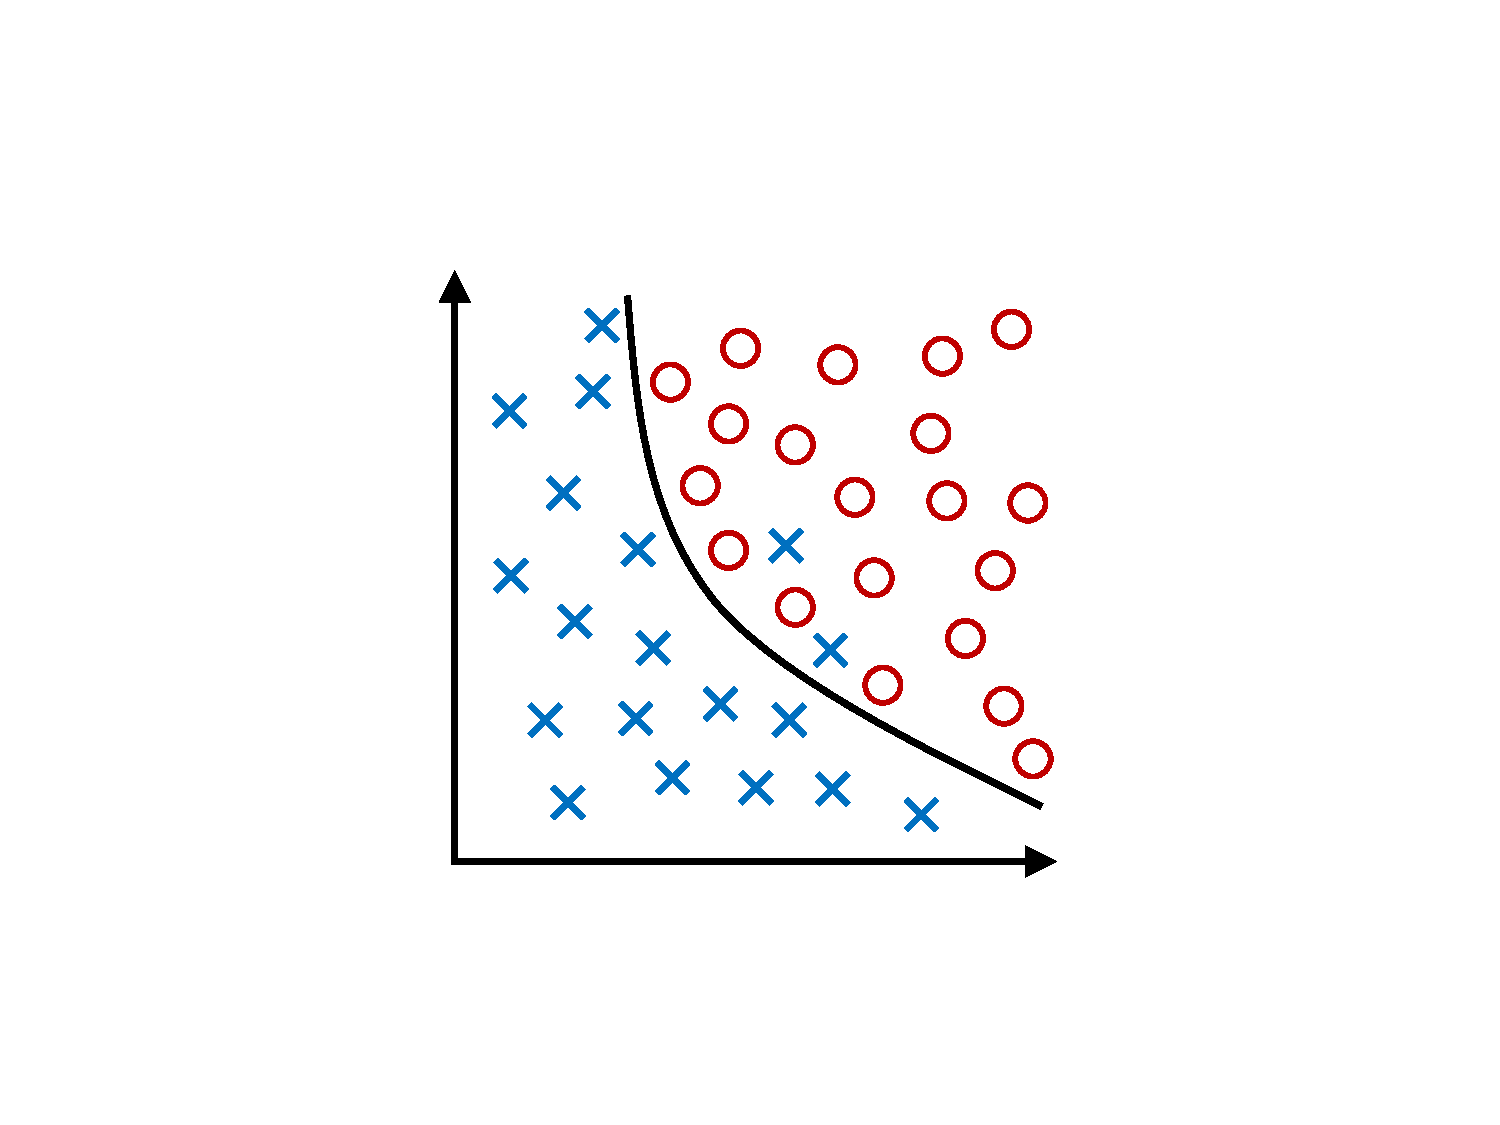
\includegraphics[width=\textwidth, page={1}, trim={6.5cm 4cm 6.5cm 4cm}, clip]{images/Overfitting}
    \caption{Appropriate fitting.}
  \end{subfigure}
  \begin{subfigure}[h!]{0.3\textwidth}
    \includegraphics[width=\textwidth, page={2}, trim={6.5cm 4cm 6.5cm 4cm}, clip]{images/Overfitting}
    \caption{Underfitting.}
  \end{subfigure}
  \begin{subfigure}[h!]{0.3\textwidth}
    \includegraphics[width=\textwidth, page={3}, trim={6.5cm 4cm 6.5cm 4cm}, clip]{images/Overfitting}
    \caption{Overfitting.}
  \end{subfigure}
  \caption{Visualisation of overfitting and underfitting in binary classification. When underfitted, the model is too simple to explain the variance in the data, yielding a high error on the training data. When overfitted, the model has memorized all training points, including outliers and produces a high error on valiation data.}
  \label{fig:fitting}
\end{figure}

Due to the ability of neural networks with sufficient depth to approximate any multidimensional function, they are naturally susceptible to overfitting \citep{tetko_neural_1995}. It is, therefore, necessary to reduce the generalisation error of a deep learning model by employing strategies to combat overfitting. Such strategies are known as regularisation techniques \citep{goodfellow_deep_2016}.

\subsubsection{Parameter Regularisation}

\subsubsection{Dropout}

Dropout is a technique to addressing the problem of overfitting in neural networks that was introduced by \citet{srivastava_dropout_2014}. It attempts reducing interdependent learning amongst neurons in a network. This is achieved by, for each iteration during the training phase, ignoring a random fraction of inputs to a given layer. An input is ignored (dropped out) by setting it to 0.

Since nodes cannot overfit on specific inputs due to them being disabled during many training iterations, the network is forced to learn reduncancies. The model is able to learn more independent features, making it more robust. During the validation and prediction phase, no dropout is applied. Therefore, nodes are able to use all inputs for predictions.

Research has shown dropout to be highly effective for the regularisation of deep neural networks with fully-connected layers \citep{wu_towards_2015}. However, the effect of dropout on convolutional layers is still subject to active research. \citet{cai_effective_2019} state that traditional dropout is mostly ineffective on convolutional layers, creating training instability. They propose four alternative dropout methods (drop-neuron, drop-channel, drop-path and drop-layer) that have been specifically designed for convolutional networks, reporting an increase in performance from all methods. 

\subsection{Evaluation techniques}

\subsubsection{Performance metrics}

Some of the most common performance metrics used to evaluate machine learning models are accuracy, precision, recall, and f1-score, which are defined as follows:

\begin{align}
  accuracy  &= \frac {TP + TN} {TP + TN + FP + FN}, \\
  precision &= \frac {TP} {TP + FP}, \\
  recall    &= \frac {TP} {TP + FN}, \\
  f1        &= \frac {2 \cdot precision \cdot recall} {precision + recall},
\end{align}

where TP is the number of true positives, FP is the number of false positives, TN is the number of true negatives and FN is the number of false negatives.

\subsubsection{Confusion matrix}

%----------------------------------------------------------------------------------------------------------------------------------

\section{Recent developments and related work}

\subsection{Applications}

\subsubsection{Pedestrian detection}

One of the most actively researched applications for deep learning and thermal imaging is pedestrian detection. Autonomous systems such as self-driving cars need to be provided with accurate environmental information to guarantee safe operation. Traditional VIS-only models are often not able to provide this accuracy \citep{zhang_how_2016}, especially under challenging conditions such as insufficient illumination, partial object occlusion or weak contrasts between objects and background in the visible light spectrum. 

The KAIST Pedestrian Detection Benchmark \citep{hwang_multispectral_2015} was introduced to provide a prediction benchmark for thermal multispectral detection models. In recent years, many novel models and methodologies have been proposed, continuously improving the state of the art \citep{konig_fully_2017}.

\subsubsection{Material recognition}

\citet{cho_deep_2018} introduce a novel technique for material type recognition using thermal imaging and deep learning. Their models is able to distinguish between 32 materials.

\subsubsection{Facial recognition}

(XXX TODO)
\citep{choi_thermal_2012}
\citep{sarfraz_deep_2017}

\subsubsection{Agriculture and food industry}

Furthermore, there are many applications of thermal imaging in agriculture and the food industry \citep{vadivambal_applications_2011}. Tasks such as food quality assessment and maturity evaluation can be automated using thermal imaging. For instance, \citet{gowen_applications_2010} report the possibility to automatically detect bruised tissue on fruit and vegetables using thermal imaging. Based upon a deep learning approach, \citet{ibarra_combined_2000} propose a noninvasive method for the estimation of the internal temperature of just-cooked meat. 


\subsection{Architectures and techniques}

\citet{dollar_fast_2014} propose a novel object detector based on aggregated channel features (ACF), achieving good object detection performance on visible light images. This approach has been adapted to multispectral data, additionally incorporating the thermal channel T, and histograms of oriented gradients (HOG) features \citep{dalal_histograms_2005} extracted from the thermal channel. This model serves as a baseline for the KAIST dataset.

\citet{wagner_multispectral_2016} evaluate early and late feature fusion methods for thermal multispectral pedestrian detection. The early fusion approach involves stacking the RGB and T channels pixel-wise into a tensor of depth 4 and feeding the result into a CaffeNet \citep{jia_caffe_2014} convolutional network. The late fusion approach feeds the RGB image and LWIR image into separate convolutional networks respectively, and merging the outputs using fully-connected layers. They conclude that, unlike the early fusion approach, the late fusion model significantly outperforms the previous state of the art ACF+T+HOG baseline.

Expanding upon the late feature fusion network introduced by \citet{wagner_multispectral_2016}, \citet{guan_fusion_2019} propose an illumination-aware approach to multispectral deep learning models. This approach is based on two-stream networks, as introduced by (XXX). After the outputs of the RGB and LWIR networks are fused, they are fed into separate networks for daytime and nighttime images. The respective predictions are then merged using illumination-aware weights. This approach achieved state-of-the-art performance on the KAIST benchmark.

%==================================================================================================================================

\chapter{Problem analysis}
\label{analysis}

\section{Data acquisition}

Collecting a multispectral dataset of sufficient quality is significantly more challenging than a dataset consisting solely of visible-light images. Specialised equipment is needed to obtain images. Using two sensors to capture LWIR and visible light introduces problems such as channel misalignment and inability to perform an optical zoom. This makes it harder to properly frame the objects of interest.

Furthermore, the majority of image classification tasks use traditional visible light imaging only. As a result, the research and resources that are available for use are much more limited.

\subsection{Sensory equipment}

Even though thermal cameras have become significantly more affordable in recent years, their resolution remains much lower than that of conventional visible-light cameras. The FLIR One Pro \footnote{\url{https://www.flir.com/products/flir-one-pro/}}, which was used for this project, is composed of two sensors:

\begin{itemize}
  \item A conventional camera for visible-light images with a resolution of $1440 \times 1080$ px.
  \item A thermal sensor with a spatial resolution of $160 \times 120$ px and a spectral range of $8 - 14 \mu m$.
\end{itemize}

The FLIR camera is, therefore, able to perceive and record electromagnetic waves in the visible-light (VIS) and long-wave infrared (LWIR) bands. Furthermore, images can be captured at a frequency of $8.7 Hz$, enabling real-time vision. Due to technical limitations, several challenges had to be overcome when working with data collected by the sensor.

Firstly, the two cameras are not spatially aligned. Furthermore, the "zoom level" or focal length of the sensors does not appear to match. A misalignment of the channels is likely to have an adverse impact on the performance of a convolutional network \citep{chappelow_improving_2008}. Therefore, the issue of image registration of the two camera outputs arises. The strategy we introduced to perform robust registration of the VIS and LWIR images is outlined in Section \ref{image_registration}.

Secondly, the vastly different resolutions of the sensors could cause problems too, as convolutional filters might struggle detecting edges and other features consistently across all channels. A possible strategy to avoid this issue is to resize the images to a common resolution. However, this means that valuable information in the VIS image might be lost and overall accuracy might be reduced. It is, therefore, necessary to evaluate the degree of information loss upon size reduction of the visible light image.

%----------------------------------------------------------------------------------------------------------------------------------

\section{Modality gap between LWIR and VIS images}
\label{modality}

As outlined in Section \ref{imaging}, LWIR and visible light are both forms of electromagnetic radiation. However, the properties of LWIR and VIS images differ significantly. \citet{sarfraz_deep_2017} refer to visible light as reflection dominant and LWIR as emission dominant radiation, resulting in a modality gap between the two corresponding sensing techniques. \citet{choi_thermal_2012} consider this modality gap a challenging problem for computer vision algorithms.

\citet{davis_background-subtraction_2007} state that thermal cameras are especially effective for object detection tasks compared to VIS cameras in low-light settings. Conversely, given sufficient illumination, visible light cameras perform better than thermal sensors if the thermal properties of objects are similar to its background. Furthermore, they state a low signal-to-noise ratio and white-black polarity calibration issues as common problems of thermal cameras.

\subsection{Noisiness}

To evaluate the relative noisiness of thermal and visible light images, a test image was taken in an indoor setting. The LWIR channel and the greyscale representation of the RBG channels can be seen in Figures \ref{fig:fourier_lwir_spatial} and \ref{fig:fourier_vis_spatial}. It is apparent that the greyscale image contains more textural details than the LWIR image. For instance, the painting above the fireplace appears as a simple gradient in the thermal band.

\begin{figure}[ht]
  \centering
  \begin{subfigure}[h!]{0.4\textwidth}
    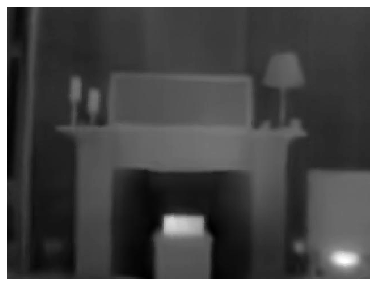
\includegraphics[width=\textwidth]{images/fourier/lwir_spatial}
    \caption{LWIR spatial domain}
    \label{fig:fourier_lwir_spatial}
  \end{subfigure}
  \begin{subfigure}[h!]{0.4\textwidth}
    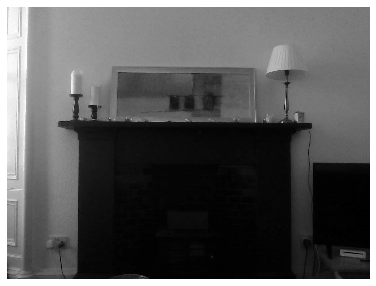
\includegraphics[width=\textwidth]{images/fourier/gray_spatial}
    \caption{VIS spatial domain}
    \label{fig:fourier_vis_spatial}
  \end{subfigure}
  \begin{subfigure}[h!]{0.4\textwidth}
    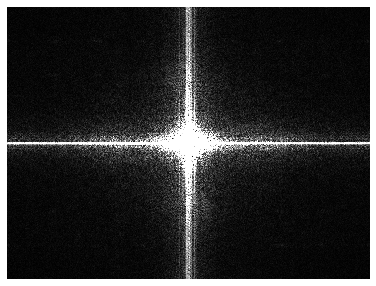
\includegraphics[width=\textwidth]{images/fourier/lwir_freq}
    \caption{LWIR frequency domain magnitude}
    \label{fig:fourier_lwir_freq}
  \end{subfigure}
  \begin{subfigure}[h!]{0.4\textwidth}
      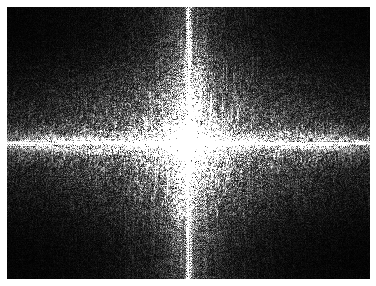
\includegraphics[width=\textwidth]{images/fourier/gray_freq}
      \caption{VIS frequency domain magnitude}
      \label{fig:fourier_vis_freq}
    \end{subfigure}
  \caption{Fast discrete fourier transform of an example LWIR and VIS image. The VIS image contains more detailed textural information, making it \textit{noisier}, as can be seen in the frequency domain.}
  \label{fig:fourier}
\end{figure}

We applied a fast fourier transform \citep{cooley_fast_1969} to both images. Fourier transforms are a method for decomposing a signal into its sinusoidal components. The original image is considered to be in the spatial domain, whereas the transformed signal represents the same information in the frequency domain. It consists of the two complex components magnitude and phase. In this case, translating into the frequency domain allows the analysis and modification of the image's geometric structure. 

Figures \ref{fig:fourier_lwir_freq} and \ref{fig:fourier_vis_freq} show the magnitude component of the aforementioned image in the frequency domain. The centre has been shifted to represent the zero frequency of the image. The distance of a point to the centre represents its frequency and the intensity its magnitude. 

It can be seen that the visible light image has a significantly higher portion of high-frequency components than its LWIR counterpart. Hence, the VIS image can be considered to be noisier than the LWIR image. This effect does not change significantly when downsampling the VIS image to the resolution of $160 \times 120$. The difference in noisiness might have an impact on the effects of convolutional filters on the LWIR and VIS images.

\subsection{Environmental conditions}

Figure \ref{fig:fourier}, furthermore, demonstrates the strengths and weaknesses of both types of sensors. Due to insufficient lighting, the whole fireplace appears as a single almost completely black surface in the VIS image. The LWIR image clearly shows two objects standing in front of the fireplace. On the other hand, the thermal image does not capture many details visible in the VIS image, such as the texture of the painting.

Hence, it appears as if a benefit of LWIR cameras compared to visible light can be achieved mainly in scenarios with a high thermal contrast and bad lighting conditions. Most mammals and avian species actively regulate their internal temperature \citep{prinzinger_body_1991} and can be picked up easily by a thermal camera. Therefore, it can be theorised that the classification of animals could be significantly improved using a thermal multispectral sensing technique.

Due to limited access to the animals, a robust evaluation of the relative performance of a multispectral model in different lighting conditions was not performed as part of this project.

%----------------------------------------------------------------------------------------------------------------------------------

\section{Transfer learning}
\label{transfer_learning_analysis}

A large amount of existing datasets is available for traditional image classification tasks. The ImageNet dataset \citep{deng_imagenet_2009}, which is used as a benchmark for many image classification models, contains over a million labelled images that can be used to train a model. Many successful deep learning models, such as AlexNet \citep{krizhevsky_imagenet_2012} and ResNet \citep{he_deep_2016} have been applied to datasets such as ImageNet.

When creating an image classifier for a new application, it is then possible to make use of a model that has been pre-trained on another dataset, such as ImageNet. This model can then be adapted by, for instance, exchanging the final fully-connected layer of that network for one that suits suits the new classification task. Finally, the model can be trained on the new dataset. This strategy is known as transfer learning and was introduced by \citet{thrun_is_1996}.

Since the features learned by early layers are often applicable across many classes and images (e.g. edge or texture features), the network generalises better, as it has been trained on an overall larger dataset. Therefore, transfer learning makes it feasible to train complex models on smaller amounts of data than usual \citep{kwasniewska_deep_2017}.

For multispectral models, this highly effective approach becomes more difficult, as much fewer datasets are available to be used off-the-shelf. Datasets for visible light and thermal data, such as the KAIST Pedestrian Detection Benchmark \citep{hwang_multispectral_2015} are available. However, They usually lack the amount of classes and general size of traditional computer vision datasets and are therefore less suitable for transfer learning tasks.

Pre-training a multispectral classifier on an VIS-only dataset is not directly possible due to the incompatible input tensor shapes ($h \times w \times 3$ compared to $h \times w \times 4$) and the resulting difference in trainable weights. Moreover, the modality gap outlined in Section \ref{modality} makes it likely that this approach would be unfeasible even if the tensor shapes were compatible.

However, there are strategies to mitigate this issue. It is possible to divide the model into two separate branches of layers that process the VIS and LWIR images individually, and perform late feature-level fusion \citep{guo_face_2017} by concatenating the respective feature maps and adding at least one fully connected layer after the concatenation. This approach can make it possible to load pretrained weights into the VIS-branch of the model without affecting the LWIR branch. During training, the LWIR-branch of the model gets trained from scratch, whereas transfer learning is simultaneously performed on the VIS-branch.

Another possible approach to enable the usage of existing off-the-shelf datasets is to perform generative image augmentation. In Section \ref{autoencoder_implementation} we explore the application of a primitive generative model for predicting the corresponding LWIR image of a known type of object from a given RGB image. Given sufficient quality of predicted images, it would then be possible to turn RGB-only images into multispectral training data.

%----------------------------------------------------------------------------------------------------------------------------------

\section{Mobile application}

This project aims to deploy the final deep learning model to a mobile edge device. This introduces many challenges related to mobile computing. Contrary to most computers, computational power on mobile devices is highly limited. Furthermore, to provide robust and reliable real-time classification, low latency between image capture and classification will be necessary. Two major strategies can be used to perform image classification on a mobile device:

\begin{enumerate}
  \item Deploy the model to a web service, upload captured frames from edge device, and retrieve the prediction.
  \item Deploy the model to the edge device and perform all computations \textit{offline} on the mobile device.
\end{enumerate}

To minimise latency, the second approach was selected. It will therefore be possible to use the application even in situations with poor connectivity. However, the necessity to perform all computational tasks on the edge device imposes many problems. The TensorFlow SDK for Java is very limited compared to the Python API. Furthermore, various image pre-processing tasks have to be performed without the standard Python data science stack that was used for training and experimentation. Many image processing libraries do not support multispectral data, further complicating image processing.

The mobile application will furthermore provide the ability to capture datasets in a convenient way, without the need to seperately extract raw RGB and LWIR images after capture.


%==================================================================================================================================

\chapter{Design}
\label{design}

\section{Dataset}

\subsection{Classes and samples}
\label{classes_samples}

Initially, a dataset consisting of 13 classes and 1042 samples was captured using the camera functionality of the mobile application. The app captures images in quick temporal succession, effectively like a video. Thus, many images are relatively similiar, as they were captured within only a few milliseconds difference. To distinguish between different bursts of images, samples were grouped into distinct subsets, each subset representing a batch of similar images.

Due to the difficulty of obtaining well-framed and unobstructed images, the data contains significant noise. Some images contain more than one animal. Furthermore, some animals were housed in closed-off shelters and were only visible behind a metal grid. This is problematic, as a classifier is likely to learn the various obstructions as features of specific classes. This can negatively impact generalisability, as the model might not be able to correctly predict unobstructed images of these classes.

Therefore, each subset was labeled as either \textit{single}, \textit{multi} or \textit{obstructed} to allow greater flexibility when selecting data for training and validation. Moreover, no distinction between genders was made. This primarily impacts the peacock class, as male and female peacocks have a very distinct appearance. Alpacas and chicken are both represented in the dataset with more than colour.

\begin{table}[ht]
  \centering
  \begin{tabular}{@{}llll@{}}
    \toprule
    \textbf{Class}  & \textbf{Dataset 1} & \textbf{Dataset 2} & \textbf{Dataset 3}  \\ \midrule
    Cat             & 205              & 0                    & 0                   \\ 
    Pig             & 30               & 0                    & 0                   \\
    Pony            & 112              & 127                  & 234                 \\
    Sheep           & 36               & 0                    & 0                   \\
    Alpaca          & 85               & 391                  & 115                 \\
    Ferret          & 33               & 0                    & 0                   \\
    Peacock         & 157              & 79                   & 0                   \\
    Hamburg chicken & 29               & 58                   & 49                  \\
    Silkie chicken  & 17               & 129                  & 83                  \\
    Muscovy duck    & 24               & 141                  & 105                 \\
    Chicken         & 138              & 151                  & 170                 \\
    Rabbit          & 32               & 16                   & 0                   \\
    Goose           & 144              & 0                    & 0                   \\ \bottomrule
  \end{tabular}
  \caption{Classes and sample size of raw animals datasets.}
  \label{table:raw_dataset}
\end{table}

Initially, the separation into training and validation data was performed using a stratified random split of all the data. As demonstrated in Section \ref{eval_train_val_split}, nearly perfect validation accuracy was achieved on this split. This is most likely a result of the aforementioned similarity of many images due to them being captured at similar times. Hence, we decided that a second independent dataset was necessary to achieve representative evaluation results. Two more datasets were captured on different days to obtain a wider range of lighting situations and background scenarios. The classes and samples of all three datasets are shown in Table \ref{table:raw_dataset}.

Finally, the subsets from the raw datasets were rearranged into a training dataset and a testing dataset. To avoid the issue of fitting and validating on too similar images, each subset was assigned whole to either of the two datasets. An attempt was made to obtain a balanced mixture of \textit{single}, \textit{multi}, and \textit{obstructed} subsets in both datasets. Furthermore, subsets that were deemed too noisy were omitted. Nonetheless, it can be assumed that achieving a perfect, representative split is difficult due to the noise in the dataset and the limited variety of contexts. The final train-validation-split is shown in Table \ref{table:train_test_dataset}. Overall, 35 subsets were assigned to the training dataset and 19 were allocated to the validation dataset.

\begin{table}[ht]
  \centering
  \begin{tabular}{@{}lllll@{}}
    \toprule
    \textbf{Class}  & \textbf{Train } & \textbf{Val.} & \textbf{Train subsets}  & \textbf{Val. subsets} \\ \midrule
    Cat             & 149             & 56                  & 3                 & 1 \\
    Pony            & 415             & 58                  & 5                 & 4 \\
    Alpaca          & 377             & 87                  & 4                 & 2 \\
    Hamburg chicken & 77              & 59                  & 3                 & 3 \\
    Silkie chicken  & 191             & 38                  & 3                 & 2 \\
    Muscovy duck    & 206             & 64                  & 6                 & 4 \\
    Chicken         & 277             & 119                 & 10                & 2 \\
    Goose           & 125             & 19                  & 1                 & 1 \\ \bottomrule
  \end{tabular}
  \caption{Sample size and subset composition of train and validation datasets.}
  \label{table:train_test_dataset}
\end{table}

The classes with low support (Pig, Sheep, Ferret, Rabbit) were dropped from the datasets, as it was deemed unlikely that a model would be able to accurately be fit on such small numbers of samples. Moreover, it was not possible to capture pictures of peacocks from a sufficient variety of contexts. Instead of training and validating on similar images of peacocks, the class was removed from the datasets. A problem that remained is the class imbalance in both datasets. Alpacas and ponies are over-represented and Hamburg chicken are significantly under-represented.

\begin{figure}[ht]
  \centering
  \begin{subfigure}[h!]{0.18\textwidth}
    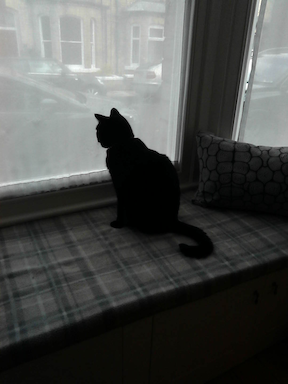
\includegraphics[width=\textwidth, trim={0cm 2.5cm 0cm 2.5cm}, clip]{images/dataset/cat/rgb.png}
    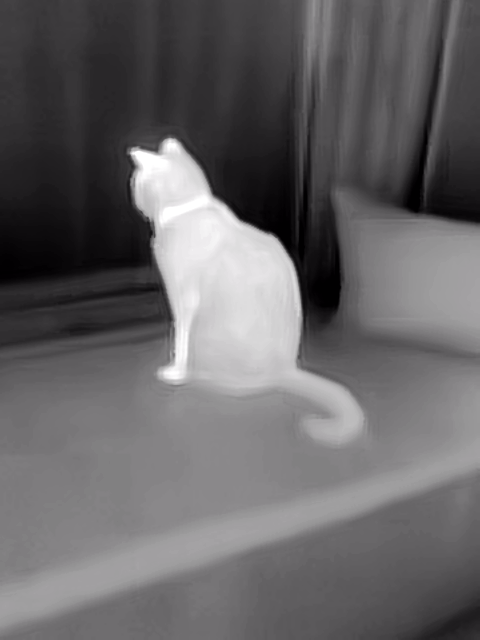
\includegraphics[width=\textwidth, trim={0cm 2.5cm 0cm 2.5cm}, clip]{images/dataset/cat/lwir.png}
    \caption{Cat}
  \end{subfigure}
  \begin{subfigure}[h!]{0.18\textwidth}
    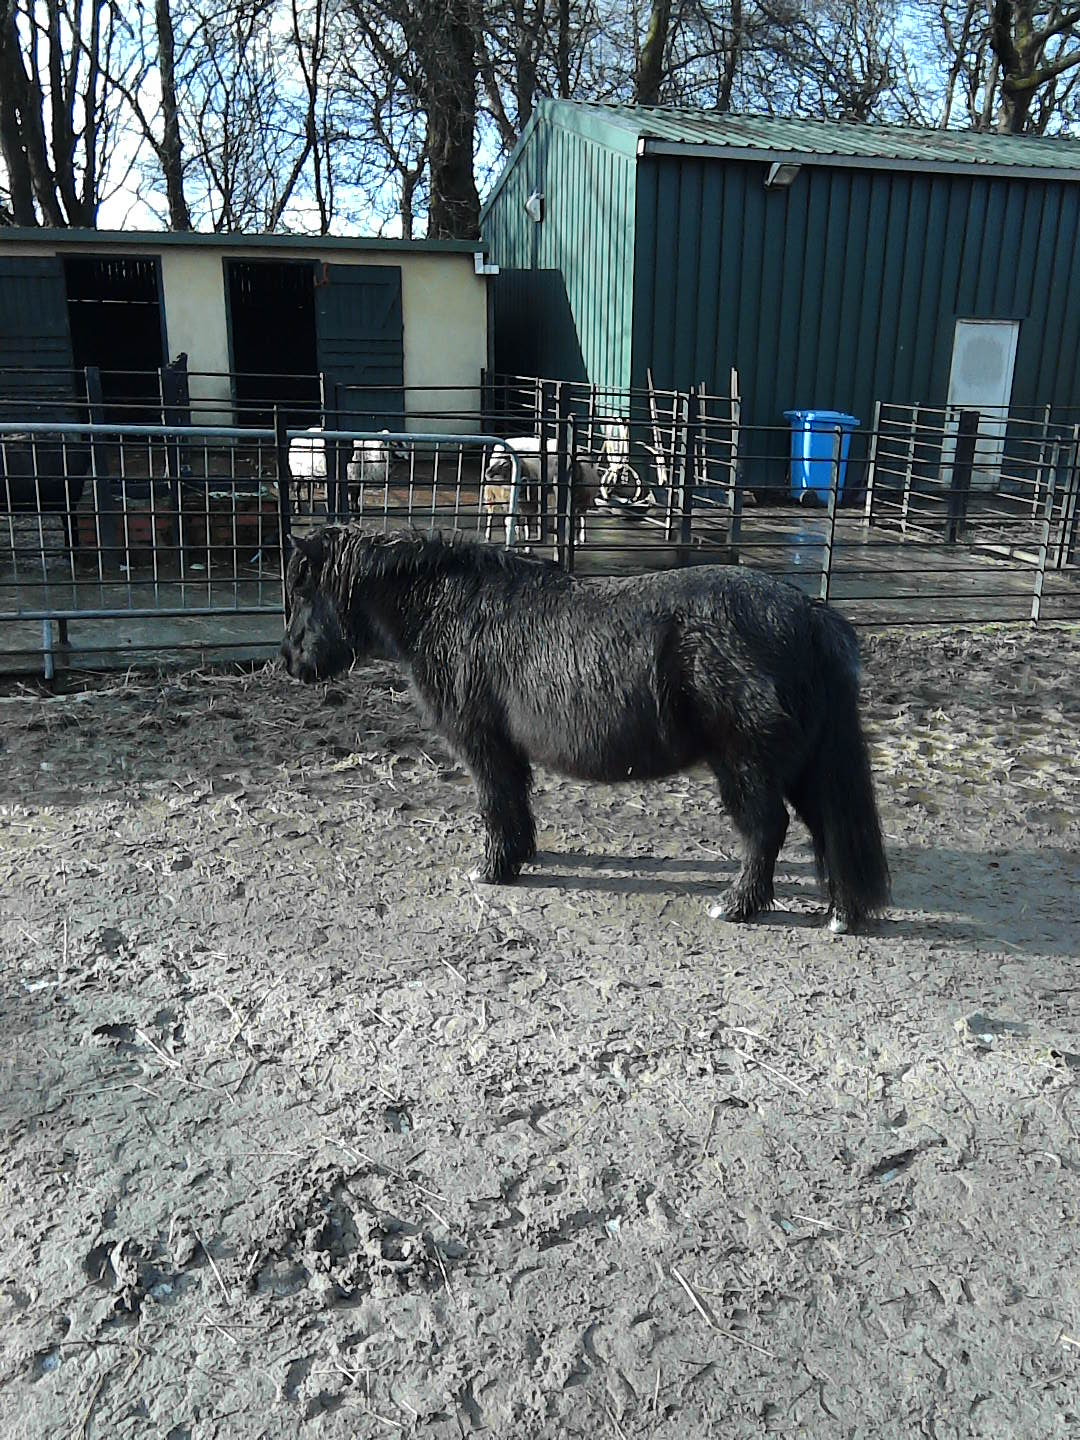
\includegraphics[width=\textwidth, trim={0cm 2.5cm 0cm 2.5cm}, clip]{images/dataset/pony/rgb.png}
    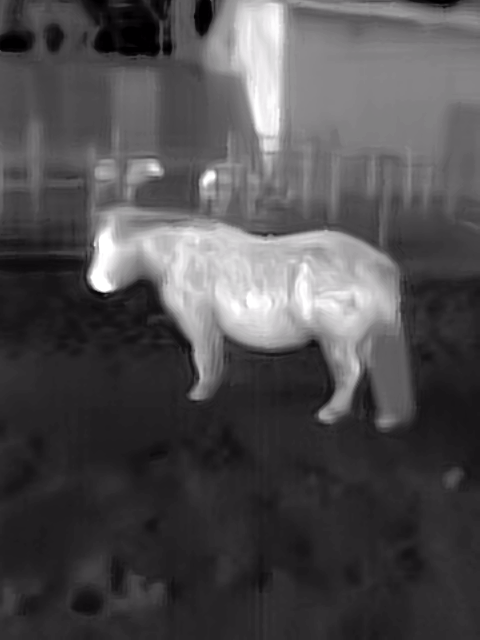
\includegraphics[width=\textwidth, trim={0cm 2.5cm 0cm 2.5cm}, clip]{images/dataset/pony/lwir.png}
    \caption{Pony}
  \end{subfigure}
  \begin{subfigure}[h!]{0.18\textwidth}
    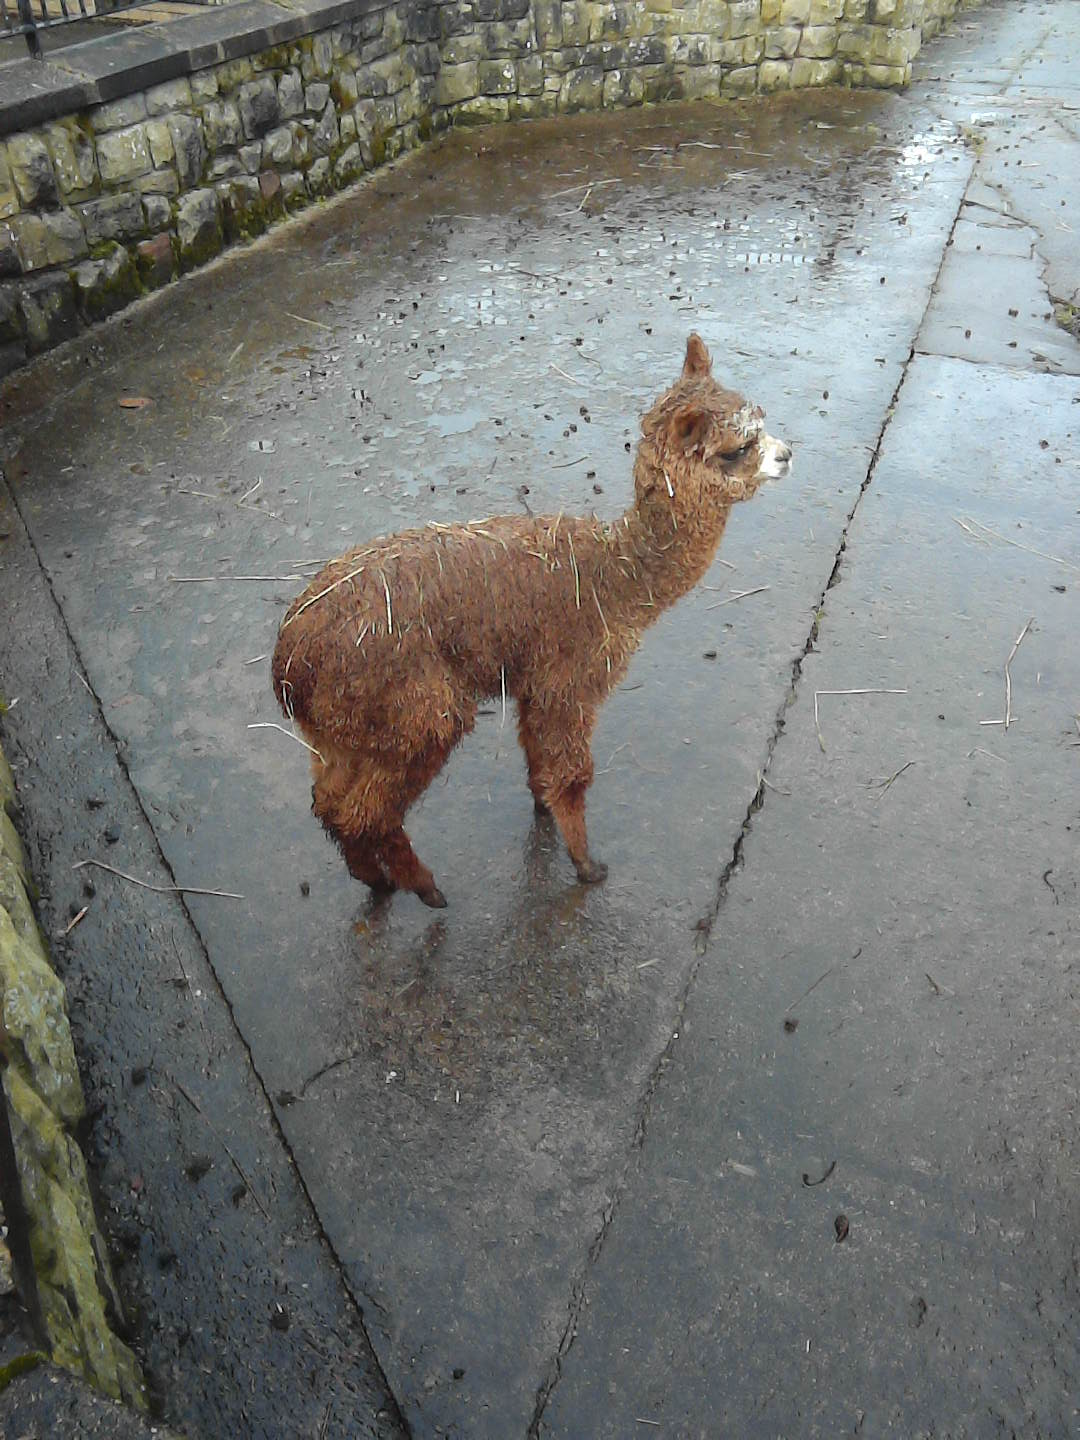
\includegraphics[width=\textwidth, trim={0cm 2.5cm 0cm 2.5cm}, clip]{images/dataset/alpaca/rgb.png}
    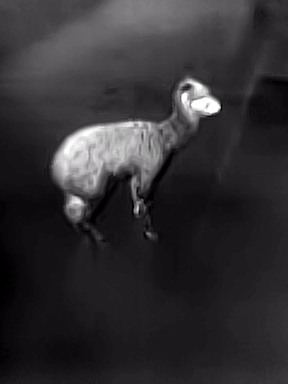
\includegraphics[width=\textwidth, trim={0cm 2.5cm 0cm 2.5cm}, clip]{images/dataset/alpaca/lwir.png}
    \caption{Alpaca}
  \end{subfigure}
  \begin{subfigure}[h!]{0.18\textwidth}
    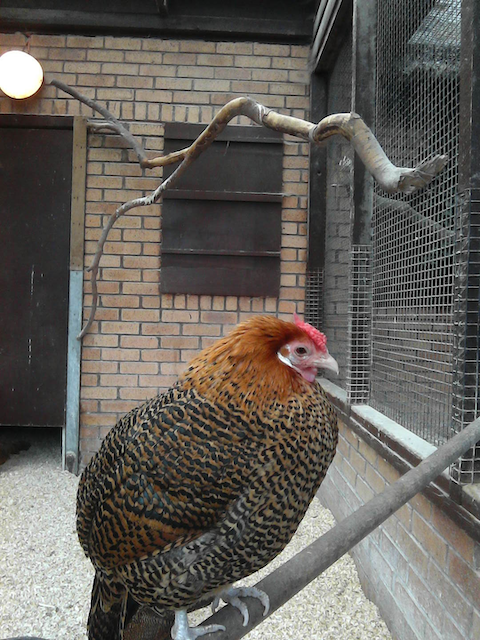
\includegraphics[width=\textwidth, trim={0cm 2.5cm 0cm 2.5cm}, clip]{images/dataset/pretty_chicken/rgb.png}
    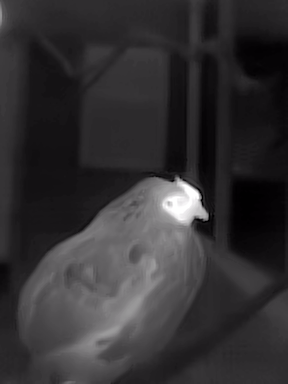
\includegraphics[width=\textwidth, trim={0cm 2.5cm 0cm 2.5cm}, clip]{images/dataset/pretty_chicken/lwir.png}
    \caption{Hamburg chicken}
  \end{subfigure}
  \\
  \begin{subfigure}[h!]{0.18\textwidth}
    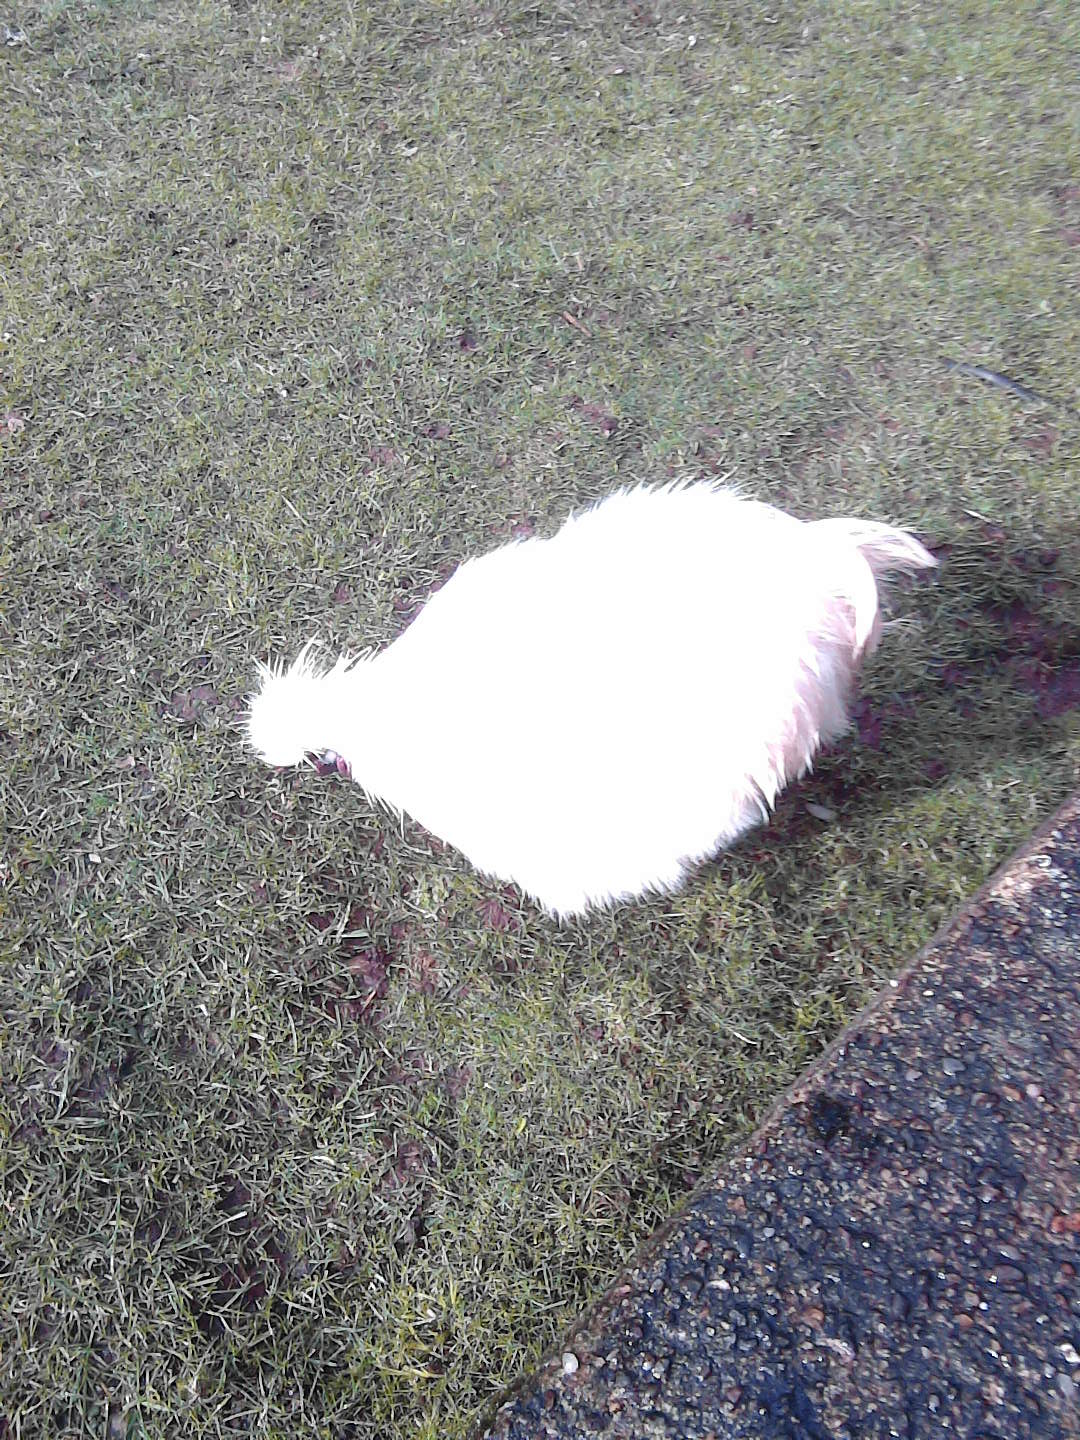
\includegraphics[width=\textwidth, trim={0cm 2.5cm 0cm 2.5cm}, clip]{images/dataset/evil_chicken/rgb.png}
    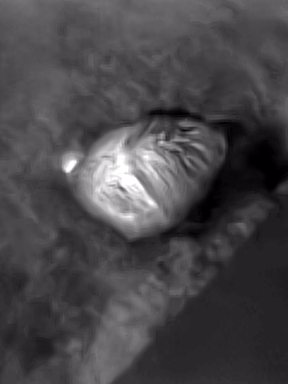
\includegraphics[width=\textwidth, trim={0cm 2.5cm 0cm 2.5cm}, clip]{images/dataset/evil_chicken/lwir.png}
    \caption{Silkie chicken}
  \end{subfigure}
  \begin{subfigure}[h!]{0.18\textwidth}
    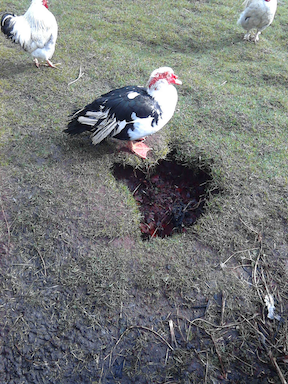
\includegraphics[width=\textwidth, trim={0cm 2.5cm 0cm 2.5cm}, clip]{images/dataset/ugly_duck/rgb.png}
    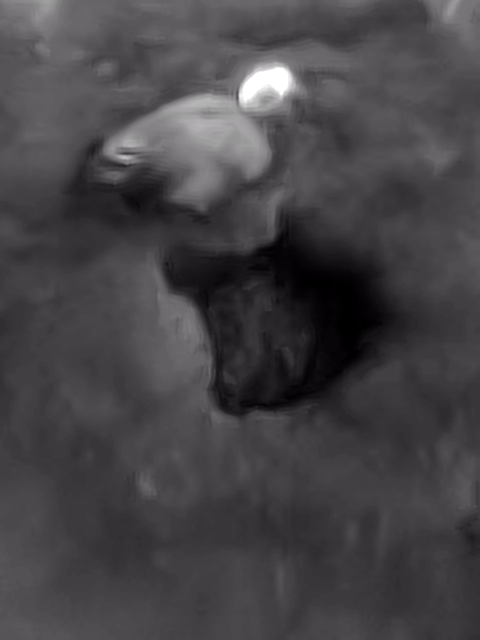
\includegraphics[width=\textwidth, trim={0cm 2.5cm 0cm 2.5cm}, clip]{images/dataset/ugly_duck/lwir.png}
    \caption{Muscovy duck}
  \end{subfigure}
  \begin{subfigure}[h!]{0.18\textwidth}
    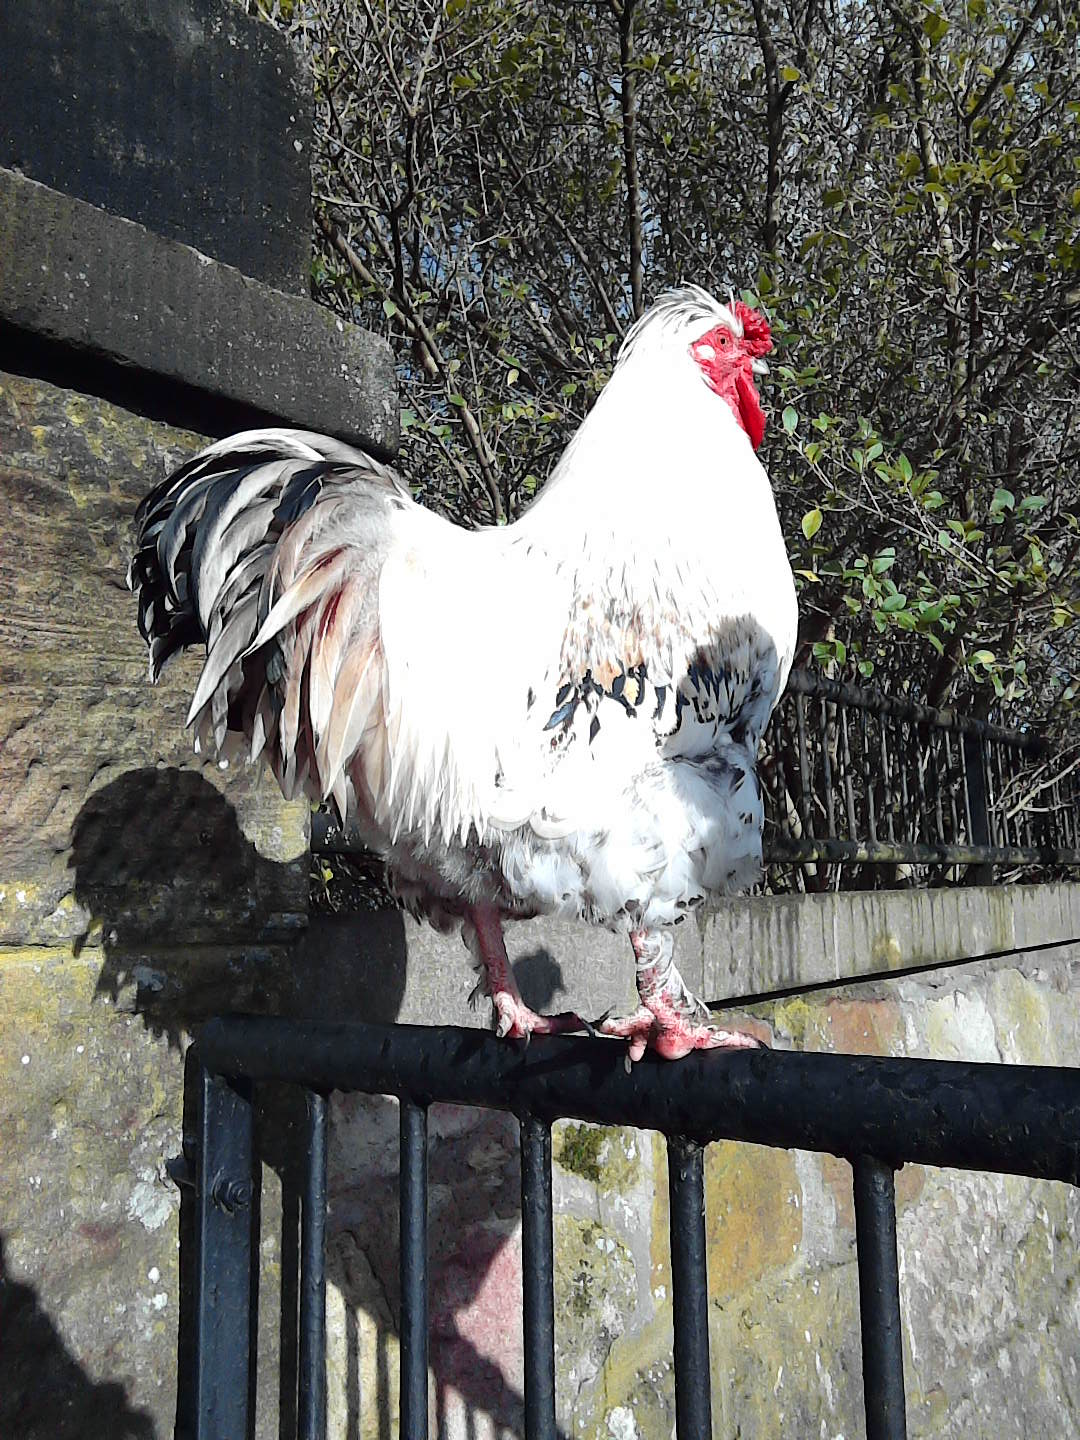
\includegraphics[width=\textwidth, trim={0cm 2.5cm 0cm 2.5cm}, clip]{images/dataset/chicken/rgb.png}
    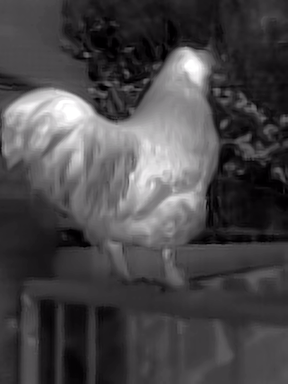
\includegraphics[width=\textwidth, trim={0cm 2.5cm 0cm 2.5cm}, clip]{images/dataset/chicken/lwir.png}
    \caption{Chicken}
  \end{subfigure}
  \begin{subfigure}[h!]{0.18\textwidth}
    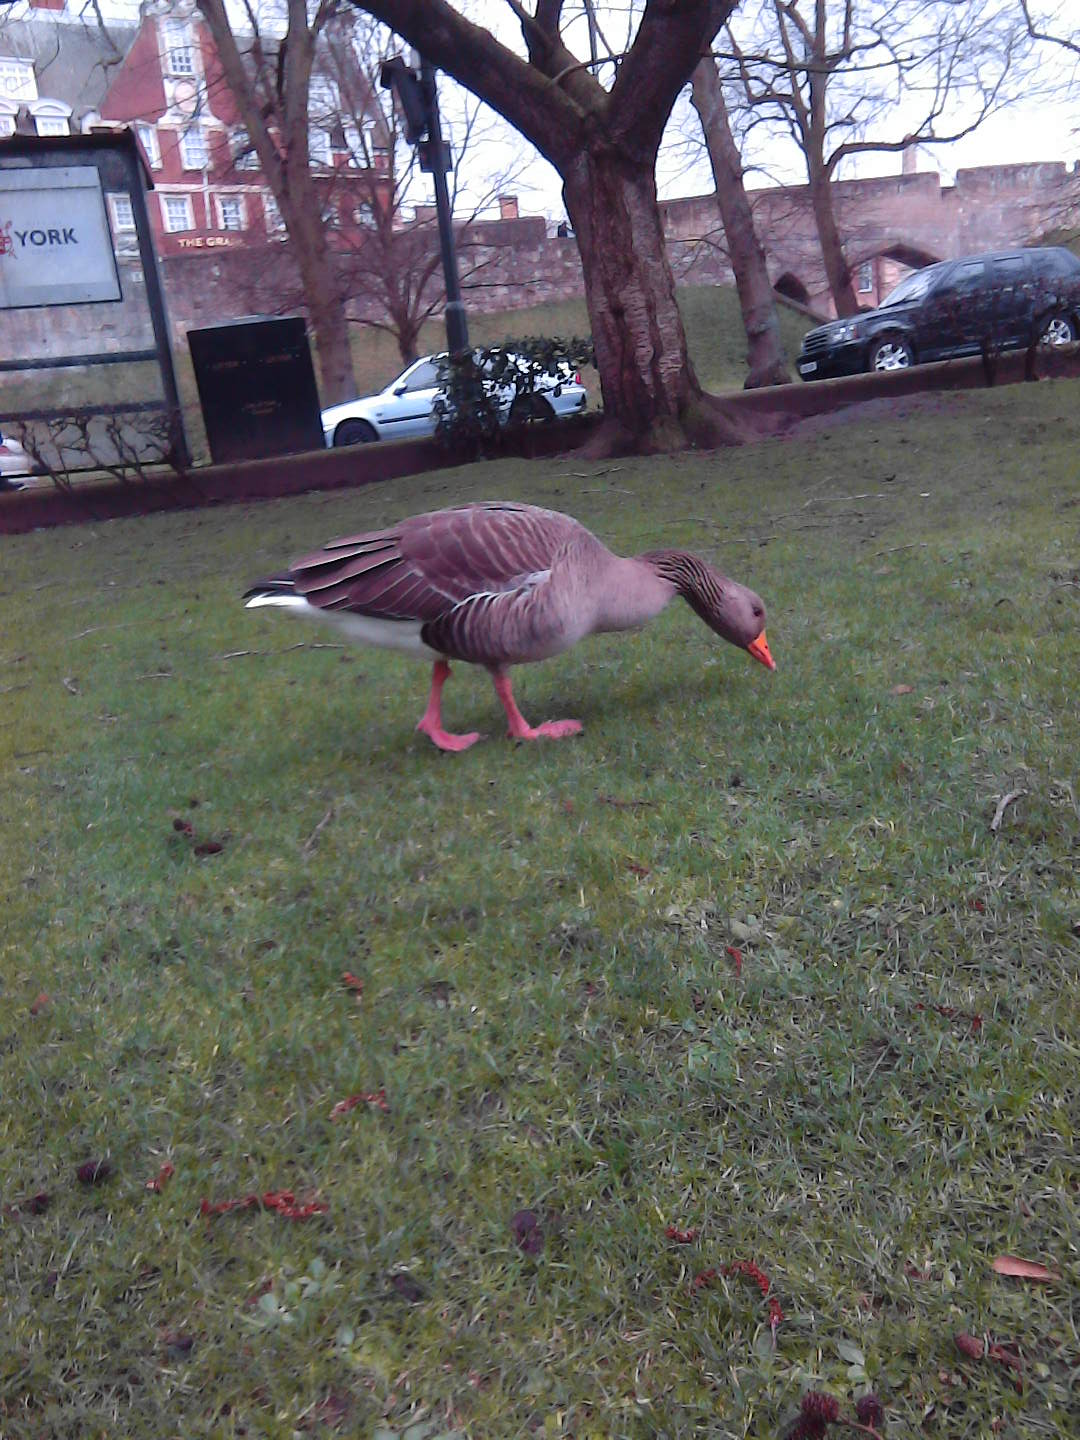
\includegraphics[width=\textwidth, trim={0cm 2.5cm 0cm 2.5cm}, clip]{images/dataset/goose/rgb.png}
    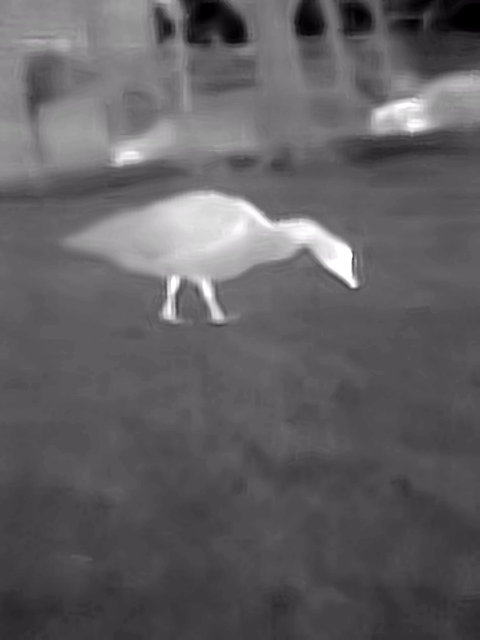
\includegraphics[width=\textwidth, trim={0cm 2.5cm 0cm 2.5cm}, clip]{images/dataset/goose/lwir.png}
    \caption{Goose}
  \end{subfigure}
  \caption{Example images for each class in the final dataset. Images have been cropped vertically.}
  \label{fig:dataset_classes}
\end{figure}

Figure \ref{fig:dataset_classes} shows example VIS and LWIR images from the training dataset. While these examples are sampeled from the idealised \textit{single} subsets without obstructions, they highlight another important caveat. Not all images could be captured at the same distance. Consequently, different animals fill different amounts of space within the images, possibly skewing classification results. An attempt was made to mitigate this issue through affine data augmentation.

\subsection{Data augmentation}

Due to the limited amount of time and resources available to the project, generating a dataset with sufficient scope and size is challenging. Since the performance of machine learning models is usually directly tied to the size and quality of the available dataset, an insufficient dataset might make it impossible to train an accurate and robust classifier \citep{fawzi_adaptive_2016}. Therefore, data augmentation was employed to artificially increase the amount of usable training samples.

\citet{mikolajczyk_data_2018} make the distinction between white-box and black-box data augmentation methods. While the latter use a form of deep learning known as Generative Adversarial Networks (GAN) to synthesise new training samples, white-box methods involve more traditional techniques, such as affine transformations. An affine transformation or affine map can accurately represent a composition of a translation and a linear map (e.g. scaling, rotation and shearing). A transformation $f(\vec{x})$ can be expressed as follows:

\begin{equation}
  f(\vec{x}) = A \vec{x} + \vec{b},
  \label{eqn:affine}
\end{equation}

where $\vec{x}$ represents the coordinates of a point to be translated, $A$ is a $2 \times 2$ linear map, and $\vec{b}$ is the translation vector. $f(\vec{x})$ can be applied to the coordinates $\vec{x}$ of every pixel, yielding a transformed image. If necessary, interpolation strategies are used to fill in gaps between the new pixels.

After evaluating various methods of data augmentation on a subset of the ImageNet dataset, \citet{perez_effectiveness_2017} conclude that traditional affine transformations alone can be very effective at improving classification performance, although GAN-based methods are promising and might yield better results.

Due to the relatively easy implementation, this project, therefore, primarily uses white-box data augmentation. However, the design and implementation of a deep-learning model generating LWIR from visible light images is discussed in Section \ref{autoencoder_implementation}. This model could be used to generate new LWIR data samples from visible light images retrieved from other sources, such as existing VIS-only computer vision datasets.

Figure \ref{fig:augmentation_affine} shows different affine transformations that were used to augment the captured dataset. The most natural transformation in this scenario is a horizontal flip, as we can assume that the objects to be classified are symmentric along the horizontal axis and the images have all been captured with similar camera orientations. Moreover, we employed randomized zooms to try to account for the varying distances that the animals were photographed from. We decided to limit the zoom factor to a small enough range to guarantee that the images still showed the whole object. Finally, we applied random rotations in the range from $-20^{\circ}$ to $20^{\circ}$ to account for slightly different camera orientations.

\begin{figure}[ht]
  \centering
  \begin{subfigure}[h!]{0.24\textwidth}
    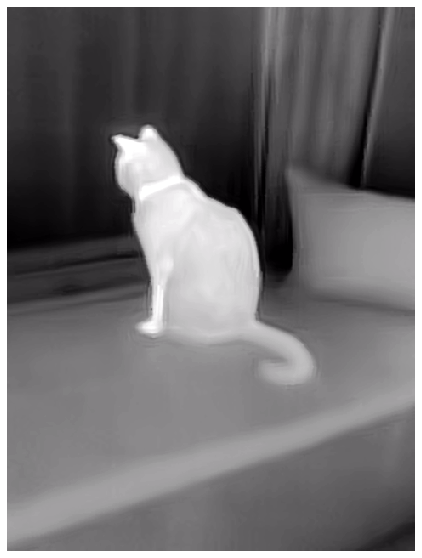
\includegraphics[width=\textwidth]{images/augmentation/original.png}
    \caption{Original image}
  \end{subfigure}
  \begin{subfigure}[h!]{0.24\textwidth}
    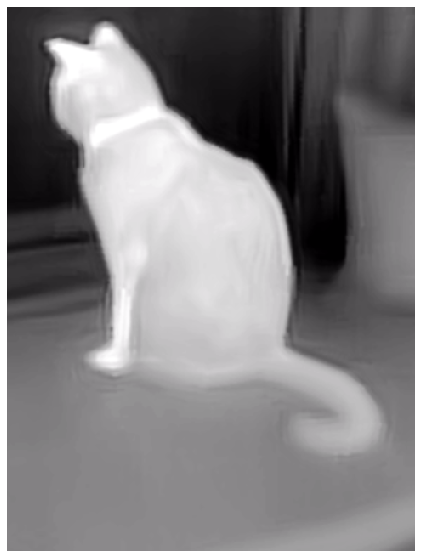
\includegraphics[width=\textwidth]{images/augmentation/zoomed.png}
    \caption{Zoomed in}
  \end{subfigure}
  \begin{subfigure}[h!]{0.24\textwidth}
    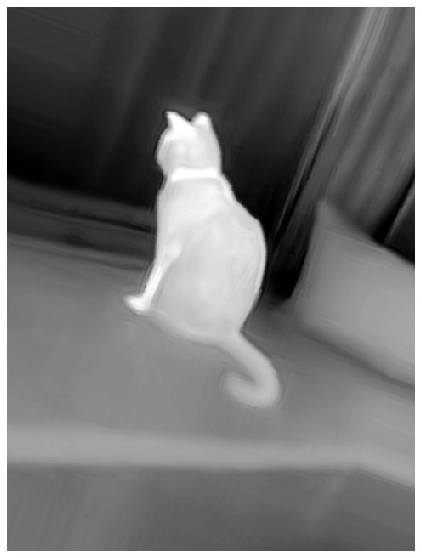
\includegraphics[width=\textwidth]{images/augmentation/rotated.png}
    \caption{Rotated $20^{\circ}$}
  \end{subfigure}
  \begin{subfigure}[h!]{0.24\textwidth}
    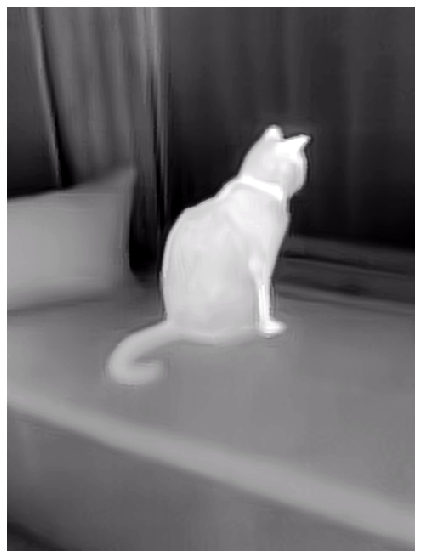
\includegraphics[width=\textwidth]{images/augmentation/flipped.png}
    \caption{Horizontally flipped}
  \end{subfigure}
  \caption{Affine data augmentation strategies applied to a sample LWIR image.}
  \label{fig:augmentation_affine}
\end{figure}

Another possible way of augmenting the data before classification is artificially drawing obstacles over the images. This approach could possibly help the model generalise better on the dataset, as a significant amount of samples from certain classes is obstructed by metal grids or foliage. However, this would require further investigation into the varying properties of visible light and LWIR images and their interaction with different types of obstacles. Hence, this approach was not implemented in this project. Instead, we decided to remove a significant part of obstructed samples from the final dataset and focused on working with higher-quality data. 

A limitation that remains with all non-generative data augmentation techniques is that the augmented samples are not fully independent from each other. The classifier only learns a very limited amount of new features from augmented samples. White-box data augmentation can, therefore, only mitigate the problem of insufficient independent samples. To achieve better generalisability, obtaining more data is preferable to augmenting existing data.

%----------------------------------------------------------------------------------------------------------------------------------

\section{Image registration}
\label{image_registration}

The images captured by the visible light camera and thermal sensor of the FLIR One Pro are not properly aligned by default. This can have adverse consequences to the classification performance of a machine learning model \citep{chappelow_improving_2008}. Thus, an algorithm for aligning the images captured by the conventional camera and LWIR camera had to be developed. The process of transforming data from different sensors into one coordinate system is commonly referred to as image registration.

To obtain workable reference samples, multiple images of three candles on a table were captured. The flames of the candles are small, bright and hot enough to function as reference points. Figure \ref{fig:linear_trans_before} displays a thresholded combined VIS and LWIR image of the three candle lights. On superficial inspection, it is apparent that the LWIR sensor appears to have a narrower field of view than the RGB camera. Hence, an attempt was made to manually align the LWIR and RGB images by cropping and rescaling the RGB image, effectively zooming in. This approach yielded moderate results, as can be seen in Figure \ref{fig:linear_trans_zoom}.

To obtain a more flexible and generalisable representation, we made use of affine transformations. As shown in Equation \ref{eqn:affine}, an affine transformation can be expressed as a linear function with parameters $A$ and $\vec{b}$. These parameters can be easily trained using a linear regression model. Therefore, the coordinates of about a dozen reference points were manually determined on the RGB and LWIR versions of some test images. These coordinates were used as features and labels for training the linear regression model. 

\begin{figure}[ht]
  \centering
  \begin{subfigure}[h!]{0.3\textwidth}
    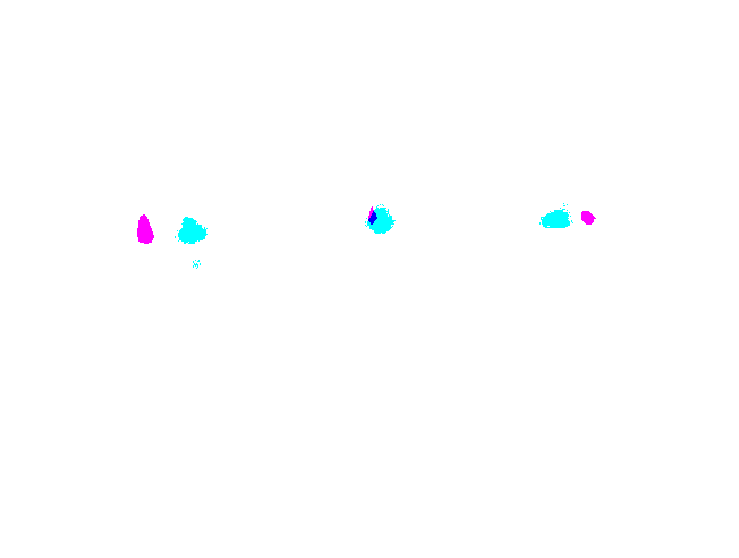
\includegraphics[width=\textwidth, trim={3.5cm 9cm 3.5cm 4.5cm}, clip, frame]{images/registration/unregistered.png}
    \caption{Before registration. The LWIR and VIS images are visibly misaligned.}
    \label{fig:linear_trans_before}
  \end{subfigure}
  \begin{subfigure}[h!]{0.3\textwidth}
    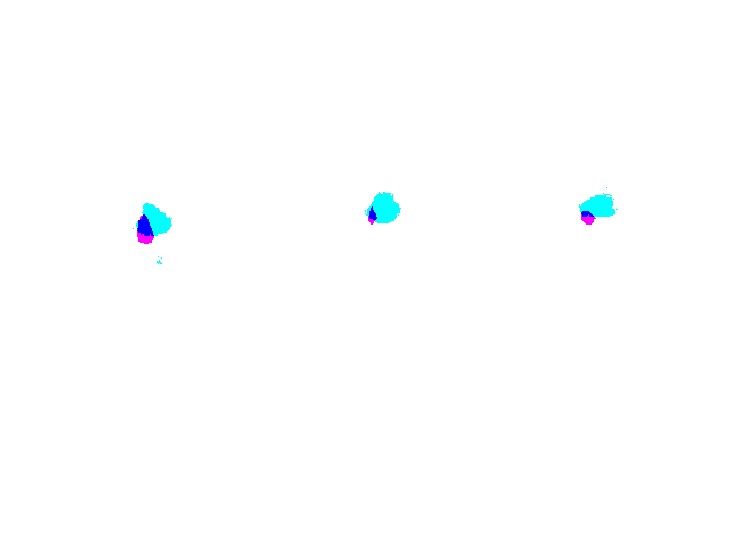
\includegraphics[width=\textwidth, trim={3.5cm 9cm 3.5cm 4.5cm}, clip, frame]{images/registration/registered_zoom.png}
    \caption{After zooming in. The images are almost aligned. A slight offset remains.}
    \label{fig:linear_trans_zoom}
  \end{subfigure}
  \begin{subfigure}[h!]{0.3\textwidth}
    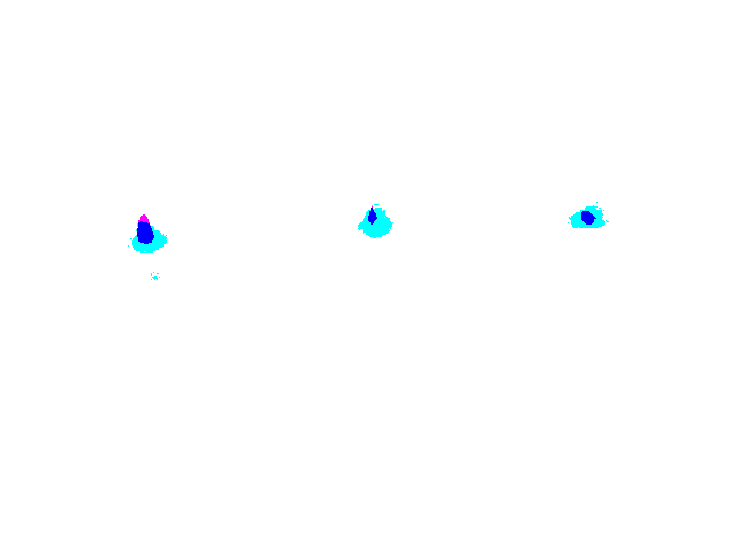
\includegraphics[width=\textwidth, trim={3.5cm 9cm 3.5cm 4.5cm}, clip, frame]{images/registration/registered_affine.png}
    \caption{After registration. The thermal signatures of the candles align with the VIS location.}
    \label{fig:linear_trans_affine}
  \end{subfigure}
  \caption{Superimposed thresholded LWIR and VIS images before and after registration. Cyan represents the grayscale version of the VIS image and the magenta represents the LWIR image.}
\end{figure}

This approach yielded acceptable results. As can be seen in Figure \ref{fig:linear_trans_affine}, the candles in the images line up. Note that the images have been thresholded to better show the alignment of the reference points.

However, defining reference points manually is a time-consuming task and the quality of alignment is dependent on the precision of those points. To quantify the accuracy of the alignment, attempts were made to use various metrics for image similarity. Such metrics could be used as loss functions for a machine learning model for automatically aligning the channels.

This task is difficult, as the properties of objects are vastly different under visible light and far infrared. Therefore, a simple intensity-based metric is unlikely to be successful in this scenario, as local intensities will vary across different channels even if the registration is perfect \citep{myronenko_intensity-based_2010}.

\subsection{Intensity-based registration metrics}

To mitigate the problem of varying intensities across different channels, \citet{chen_normalized_2018} introduce the normalized total gradient (NTG) metric for multispectral imaging systems, which is defined as follows:

\begin{equation}
  NTG(f, f_R) = \frac{\sum_l |\nabla_l \{f - f_R\}|}{\sum_l | \nabla_l f | + \sum_l | \nabla_l f_R|},
\end{equation}

where $f$ and $f_R$ are the channel images to be compared, $\nabla_l$ represents the gradient computation along the direction $l \in \{x, y\}$, and $| \cdot |$ denotes the L1-norm.

In other words, to obtain NTG one computes the sum of the $x$- and $y$-gradients of the difference of the two channels, and normalises the result by dividing over the sum of gradients of the individual channels.

The metric is based on the assumption that the gradient of the channel difference image becomes sparser as the alignment improves. Figure \ref{fig:gradient_distribution} shows that this is hardly the case for images captured by the LWIR camera, as opposed to the baseline of comparing the red and green channels from the VIS camera.

The resolution of the LWIR image files, as output by the FLIR camera, is $640 \times 420$ px, although the actual resolution of the sensor is only $160 \times 120$. Thus, when downsampling the VIS image to $640 \times 420$ px, edges are still much sharper than for the corresponding LWIR image. However, downsampling both images to the native resolution of the LWIR camera did not yield better results.

\begin{table}[ht]
  \centering
  \begin{tabular}{@{}lll@{}}
  \toprule
  \textbf{Test configuration}                             & \textbf{Misaligned} & \textbf{Aligned} \\ \midrule
  LAB intensity of VIS vs LWIR (640x480)     & 0.9984              & 0.9987           \\
  LAB intensity of VIS vs LWIR (160x120)    & 0.9974              & 0.9986           \\
  LAB intensity of VIS vs LWIR (after LoG with $\sigma=2$) & 0.9970              & 0.9973           \\
  (Baseline) Red vs green channels of RGB (160x120)                  & 0.6245              & 0.0303           \\ \bottomrule
  \end{tabular}
  \caption{Normalized Total Gradient before and after channel alignment}
  \label{table:registration_ntg}
\end{table}

Moreover, an attempt at smoothing both images before calculating the NTG was made by applying the Laplacian of Gaussian (LoG) filter with $\sigma=2$ to both images. As can be seen in Table \ref{table:registration_ntg}, this approach was not successful either. To verify that our implementation of the metric was indeed working correctly, we computed the NTG between the red and green channel of the visible light image before and after applying a random affine transformation to the green channel. As shown in Table \ref{table:registration_ntg}, the metric is very effective for the red-green-channel baseline. 

Considering these results, we concluded that NTG does not appear to be a suitable metric for this particular registration problem. Since the algorithm is effective on the baseline, it is possible that the properties of the LWIR and RGB channels are too different for an intensity-based approach.

\begin{figure}[ht]
  \centering
  \begin{subfigure}[h!]{0.45\textwidth}
    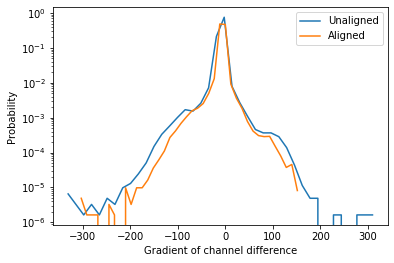
\includegraphics[width=\textwidth]{images/registration/gradient_distribution.png}
    \caption{LAB intensity of visible light image vs thermal intensity at $640 \times 420$ px}
    \label{fig:gradient_distribution}
  \end{subfigure}
  \begin{subfigure}[h!]{0.45\textwidth}
    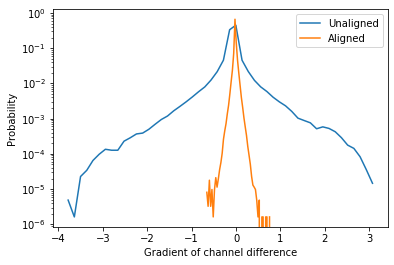
\includegraphics[width=\textwidth]{images/registration/gradient_distribution_red_green.png}
    \caption{Red channel intensity vs green channel intensity at $640 \times 420$ px}
    \label{fig:gradient_distribution_red_green}
  \end{subfigure}
  \caption{Distribution of gradients of the channel difference image before and after alignment using affine transformation.}
\end{figure}

\subsection{Texture-based registration}

Having demonstrated that intensity-based metrics appear to be inadequate to quantify the registration of visible light and LWIR images, an approach based on image texture features, as proposed by \citet{jarc_graz_2007} was tested. 

The method uses pairs of 1-D filter masks as introduced by \citet{laws_rapid_1980} to detect level, edge, spot and ripple features. These filters can be applied horizontally and vertically. In our implementation, all possible filter pairs were evaluated.

After convoluting both the LWIR and RGB images with the filters, the results were turned into texture energy images by performing a convolutional sum-operation of absolute values using a $15 \times 15$ kernel and applying a threshold of $\pm 3 \sigma$. Figure \ref{fig:le_filter} shows corresponding VIS and LWIR images after applying the level kernel horizontally and the edge kernel vertically.

\begin{figure}[ht]
  \centering
  \begin{subfigure}[h!]{0.25\textwidth}
    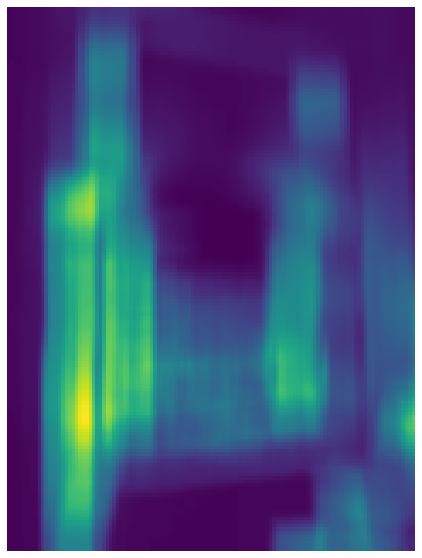
\includegraphics[width=\textwidth]{images/registration/filtered_le_rgb.png}
    \caption{VIS}
  \end{subfigure}
  \begin{subfigure}[h!]{0.25\textwidth}
    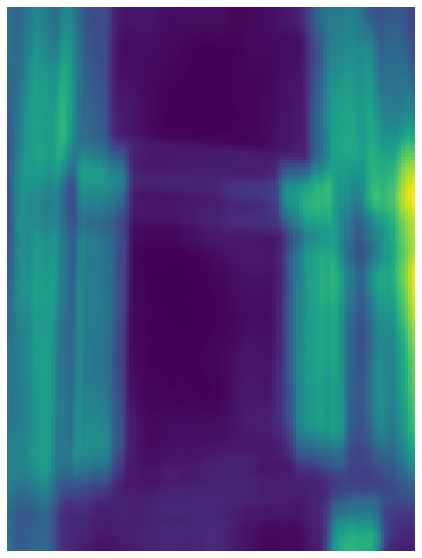
\includegraphics[width=\textwidth]{images/registration/filtered_le_lwir.png}
    \caption{LWIR}
  \end{subfigure}
  \caption{Effect of LE-Kernel \citep{laws_rapid_1980} on visible light and LWIR images.}
  \label{fig:le_filter}
\end{figure}

Finally, the mutual information (MI) of the resulting LWIR and RGB images was calculated as follows:

\begin{equation}
  MI(A,B) = H(A) + H(B) - H(A,B),
\end{equation}

where $H(X) = - \sum_{x \in X} p(x) \cdot \log_2 p(x)$ is the entropy of $X$ and $H(X,Y)$ represents the joint entropy of $X$ and $Y$.

We then averaged the MI scores obtained by all 1-D filter pairs to obtain a single metric. For the test images, the MI score did not appear to change consistently when aligning the images. Furthermore, none of the individual MI values for the different filter combinations behaved reliably across all images. Hence, we concluded that this strategy is not suitable for this registration problem.

\subsection{Mean distance}

Since neither intensity-based nor texture-based approaches produced satisfactory results, we concluded that an automatic registration of the visible light and LWIR images was unfeasible without extensive further research. Therefore, to be able to guarantee an acceptable alignment quality across the whole dataset, we resorted back to manual alignment.

For this purpose, 97 reference points were manually determined from the training data. One image was drawn from each of the 35 subsets, ensuring that all available camera orientations and perspectives were incorporated into the model. The coordinates were rescaled to $120 \times 160$, which is the desired input resolution for the CNNs. Subsequently, by fitting a linear regression model, the transformation parameters were determined to be: 

\begin{equation}
  A = \begin{pmatrix}
    1.260 & -0.016  \\
    0.020 & 1.192
  \end{pmatrix}, \ 
  \vec{b} = \begin{pmatrix}
    -14.619  \\
    -18.660
  \end{pmatrix}.
\end{equation}

Prior experiments showed that the required transformation seems to be mostly consistent across different images. Device orientation appears to be the only factor with a large impact on the required transformation. To avoid this problem, all images were captured in portrait mode. Figure \ref{fig:registration_relationship} shows the relationship between the re-scaled visible light and LWIR coordinates across both dimensions. The relationship appears to be linear. However, it can be seen that the gradient for the relationship of horizontal coordinates is slightly steeper than for the vertical coordinates. This supports the necessity to perform an affine transformation, as opposed to just zooming in.

\begin{figure}[ht]
  \centering
  \begin{subfigure}[t]{0.45\textwidth}
    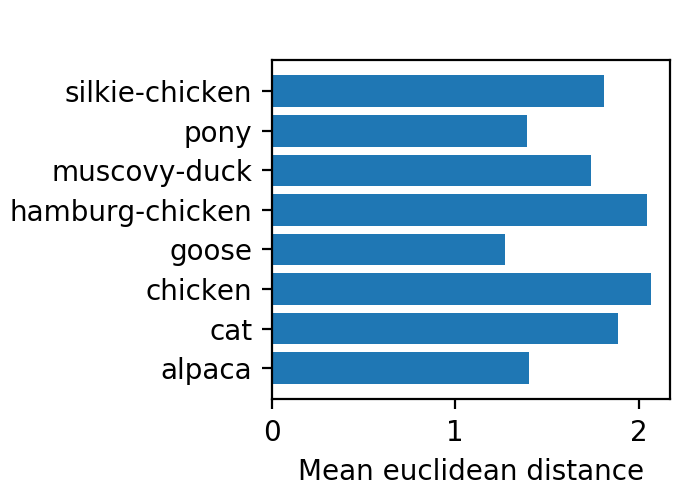
\includegraphics[width=\textwidth]{images/registration/error}
    \caption{Mean distance between predicted and actual LWIR coordinates.}
    \label{fig:registration_error}
  \end{subfigure}
  \begin{subfigure}[t]{0.4\textwidth}
    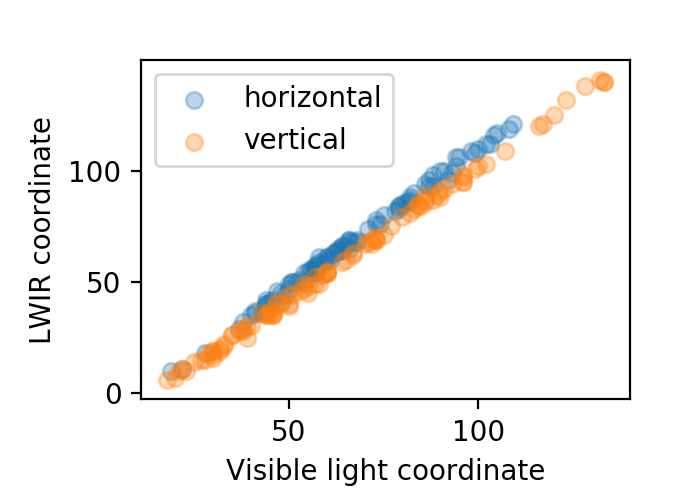
\includegraphics[width=\textwidth]{images/registration/x_y}
    \caption{Relationship between reference points in VIS and LWIR images.}
    \label{fig:registration_relationship}
  \end{subfigure}
  \caption{Manual alignment results. (XXX fix alignment)}
\end{figure}

To quantitatively evaluate whether the transformation parameters generalise across all images, the mean euclidean distance between the actual LWIR coordinates and the ones predicted by the regression model was computed for every class in the dataset. The results can be seen in Figure \ref{fig:registration_error}. The highest mean distance is around 2, which we consider small considering the image resolution. It is very likely that these errors are due to noise in the manually determined reference points. The mean distance across all reference points in the dataset was determined to be around 1.777 with $\sigma = 0.589$.

When using convolutional kernels with a small size, such as $3 \times 3$, this distance could be problematic, as edges and other features might not be picked up consistently across channels. Therefore, an attempt was made to use larger kernels in the initial convolutional layer to mitigate this potential problem.

%----------------------------------------------------------------------------------------------------------------------------------

\section{Classifiers}

As concluded in \ref{fig:augmentation_affine}, the spatial and intensity properties of RGB and LWIR images are significantly different. Due to the registration problem and the different intensity distributions, a stacked multispectral approach is unlikely to produce satisfactory results. Consequently, we decided to implement six different configurations of every CNN and evaluate the results separately.

\begin{figure}[ht]
  \centering
  \begin{subfigure}[h!]{0.3\textwidth}
    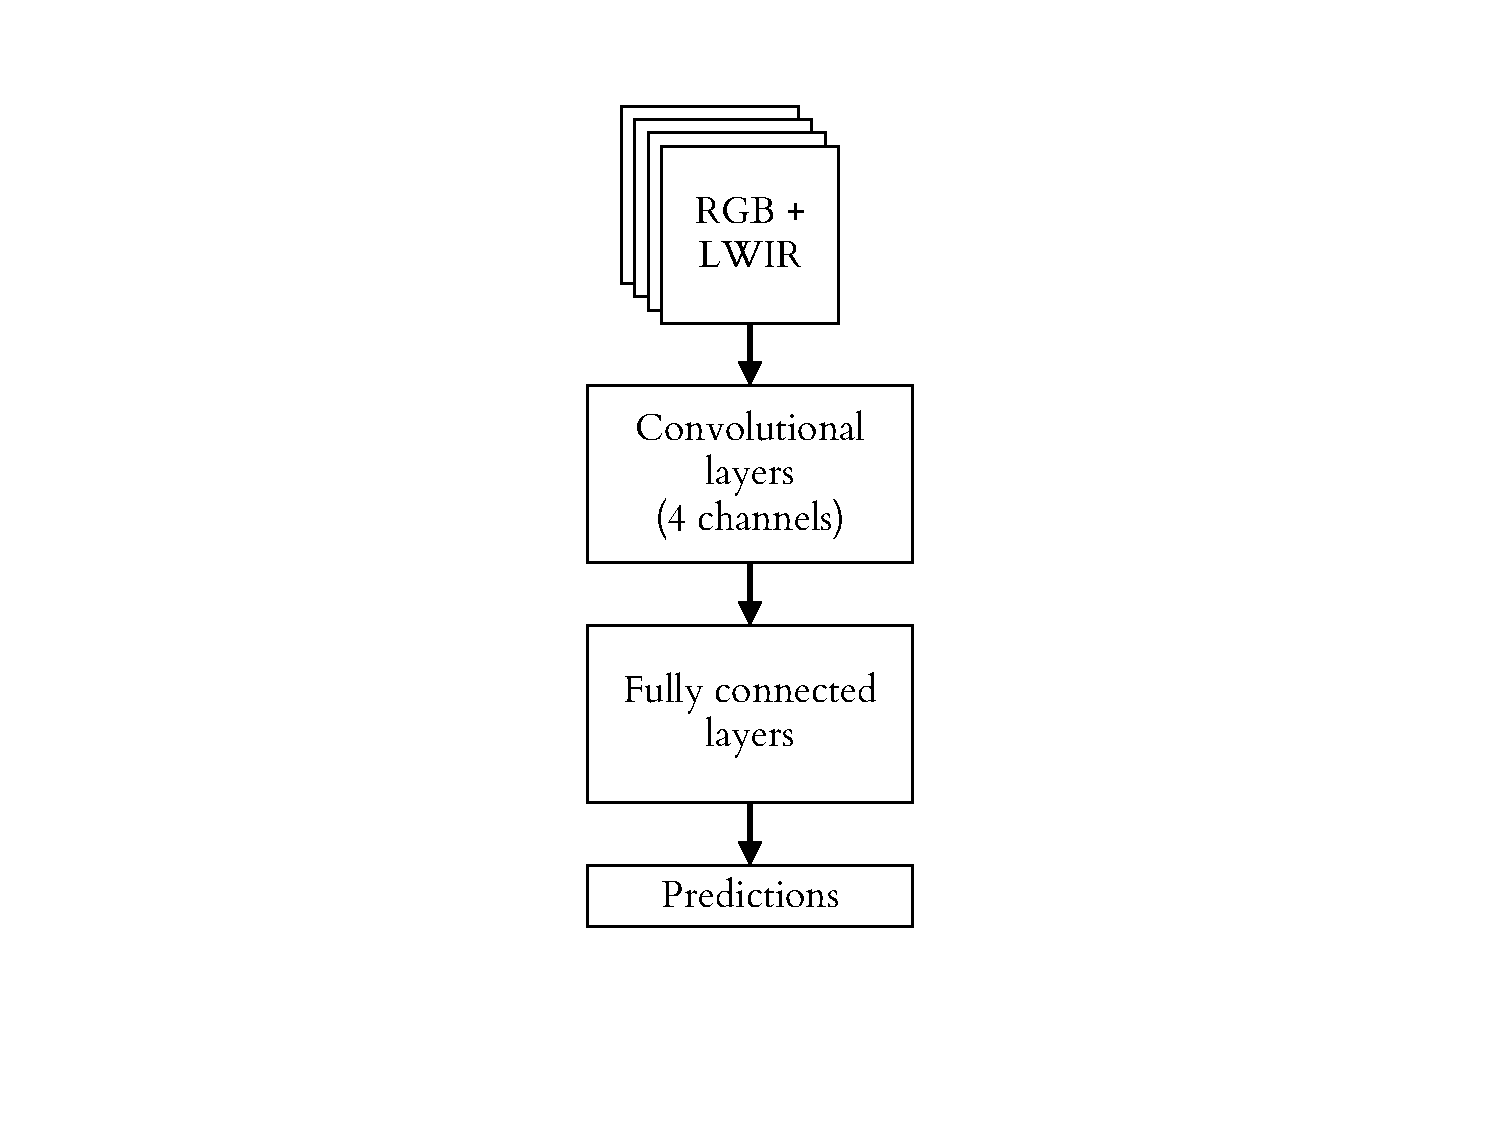
\includegraphics[width=\textwidth, page={1}, trim={6.5cm 2.2cm 6.5cm 1.5cm}, clip]{images/models/archs}
    \caption{Pixel fusion configuration.}
    \label{fig:arch_stacked}
  \end{subfigure}
  \begin{subfigure}[h!]{0.3\textwidth}
    \includegraphics[width=\textwidth, page={2}, trim={6.5cm 2.2cm 6.5cm 1.5cm}, clip]{images/models/archs}
    \caption{Score fusion configuration.}
    \label{fig:arch_combsum}
  \end{subfigure}
  \begin{subfigure}[h!]{0.3\textwidth}
    \includegraphics[width=\textwidth, page={3}, trim={6.5cm 2.2cm 6.5cm 1.5cm}, clip]{images/models/archs}
    \caption{Late feature fusion configuration.}
    \label{fig:arch_fusion}
  \end{subfigure}
  \caption{Implemented neural network configurations excluding RGB-only, LWIR-only and grayscale.}
  \label{fig:archs}
\end{figure}

\begin{enumerate}
  \item An RGB-only implementation similar to the default implementation of most networks. This will be used as a baseline.
  \item An LWIR-only implementation.
  \item A greyscale implementation. This will calculate the mean across the three colour channels of the RGB image, yielding a single-channel greyscale image. The purpose of this model will be to evaluate the benefits and drawbacks of using all three colour channels.
  \item A single-branch, pixel fusion implementation. The RGB and LWIR channels are stacked into a tensor of shape $({batch\ size} \times width \times height \times 4)$. This tensor is then fed into the network, yielding a prediction. This configuration is shown in Figure \ref{fig:arch_stacked}.
  \item A multi-branch implementation with late feature-level fusion, as shown in Figure \ref{fig:arch_fusion}. Here, the RGB and LWIR images are fed into separate branches of convolutional layers. Finally, the respective outputs are flattened, concatenated and fed into the fully-connected layers at the end of the network.
  \item A multi-branch score-level fusion implementation with voting classifiers. Similarly to the late feature-fusion implementation, the VIS and LWIR images are run through seperate network branches. However, the branches have their own individual fully-connected layers, which produce separate predictions. The final output is the weighted mean of these two predictions. The relative weights of the branches can be treated as trainable parameters. This configuration can be seen in Figure \ref{fig:arch_combsum}.
\end{enumerate}

Following the conclusion of \citet{wagner_multispectral_2016} about early and late feature fusion, this project aims to evaluate the performance of pixel-based fusion, feature-level fusion and score-level-based fusion classifiers \citep{guo_face_2017}. We chose the RGB-only networks as a baseline, as most image classification models rely solely on visible light.

Furthermore, multiple different CNN designs were evaluated. At first, a custom neural network was designed and implemented. In addition, we implemented modified versions of AlexNet and ResNet, two networks commonly used for image classification tasks. 

Note that the following architecture diagrams (Figures \ref{fig:alexnet} and \ref{fig:resnet}) show the RGB-only configurations. The other configurations can be derived from these and the architectural visualisation in Figure \ref{fig:archs}.

\subsection{Custom CNN}

A custom CNN architecture as shown in Figure \ref{fig:customnet} was implemented. The network follows a common design pattern for image classifiers, chaining multiple convolutional and pooling layers with increasing amounts of filters, followed by one or more fully-connected layers. 

\begin{figure}[ht]
  \centering
  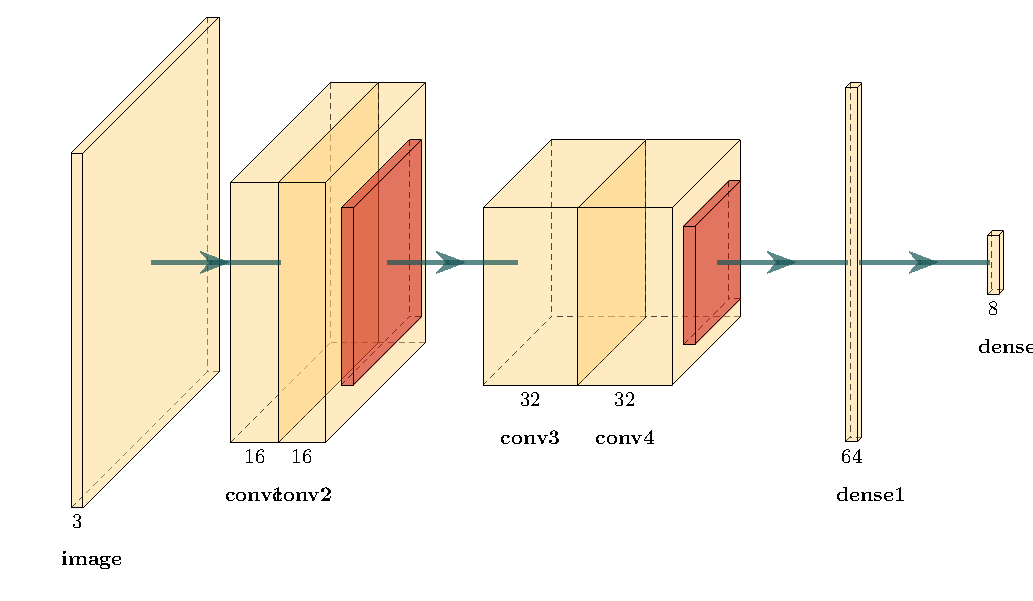
\includegraphics[width=0.7\textwidth]{images/models/customnet}
  \caption{Architecture of custom neural network.}
  \label{fig:customnet}
\end{figure}

Our model consists of two multi-layer blocks. Each block is composed of two convolutional layers, a leaky ReLU activation function, and a max pooling layer. We chose the kernel sizes to be $3 \times 3$ and $11 \times 11$ in the first block, and $3 \times 3$ and $7 \times 7$ in the second block. Following the convolutional blocks, we add a fully connected (FC) layer and an output layer with softmax activation. 

Overall, the model has $117\,592$ trainable weights. This architecture was designed as a low-end model with relatively few parameters that is fast to train and evaluate.

\subsection{AlexNet}

AlexNet was first introduced by \citet{krizhevsky_imagenet_2012}, winning the ImageNet Large Scale Visual Recognition Challenge (ILSVRC). Significantly outperforming the state-of-the-art traditional image classification models of its time, AlexNet is considered a significant breakthrough in computer vision \citep{alom_history_2018}.

The architecture of AlexNet consists of an initial convolutional layer with a relatively large kernel size of $11 \times 11$, followed by a max pooling layer. This is followed by a second block of convolutional and pooling layers. The kernel size of the second convolutional layer is $5 \times 5$. Subsequently, three convolutional layers with $3 \times 3$ kernels are applied, followed by another pooling layer. Finally, the output is fed into two subsequent fully connected layers, followed by an output layer with a softmax activation function.

We decided to evaluate an implementation of AlexNet due to various factors. Firstly, the model has delivered good results on many image classification tasks. Simultaneously, its architecture can be considered shallow compared to most modern-day networks. This makes it likely that AlexNet will be able to run with low latency on a mobile edge device. Finally, the first convolutional layer of AlexNet has a very large kernel compared to most modern-day networks. This might help mitigate the aforementioned misalignment problem.

\begin{figure}[ht]
  \centering
  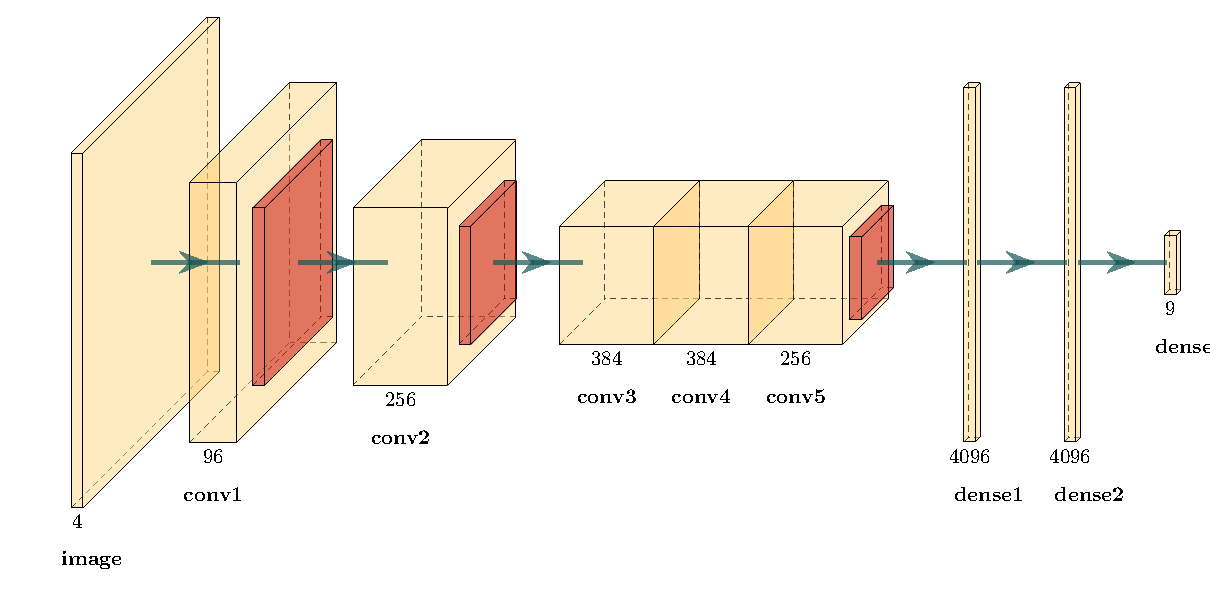
\includegraphics[width=0.9\textwidth]{images/models/alexnet}
  \caption{Neural network architecture of AlexNet.}
  \label{fig:alexnet}
\end{figure}

Our implementation of AlexNet, as shown in Figure \ref{fig:alexnet} diverges slightly from the original. Due to a lower input resolution and a smaller number of resulting parameters, the FC layers at the end of the network only have 1024 instead of 4096 parameters each. Furthermore, we included dropout layers after both FC layers to combat overfitting. In total, our AlexNet implementation has $7\,951\,752$ trainable parameters in the RGB-only configuration.

\subsection{ResNet}

Since the initial introduction of AlexNet, many more CNN-architectures have been developed. \citet{simonyan_very_2015} propose VGG, a neural network with a substantially increased number of convolutional layers. They demonstrate that deeper networks are more likely to perform well on image classification tasks than shallow architectures \citep{alom_history_2018}.

ResNet was developed by \citet{he_deep_2016}. Winning the 2015 ILSVRC, ResNet is considered a state-of-the-art neural network for image classification. It makes heavy use of a novel design component known as residual block. 

\begin{figure}[ht]
  \centering
  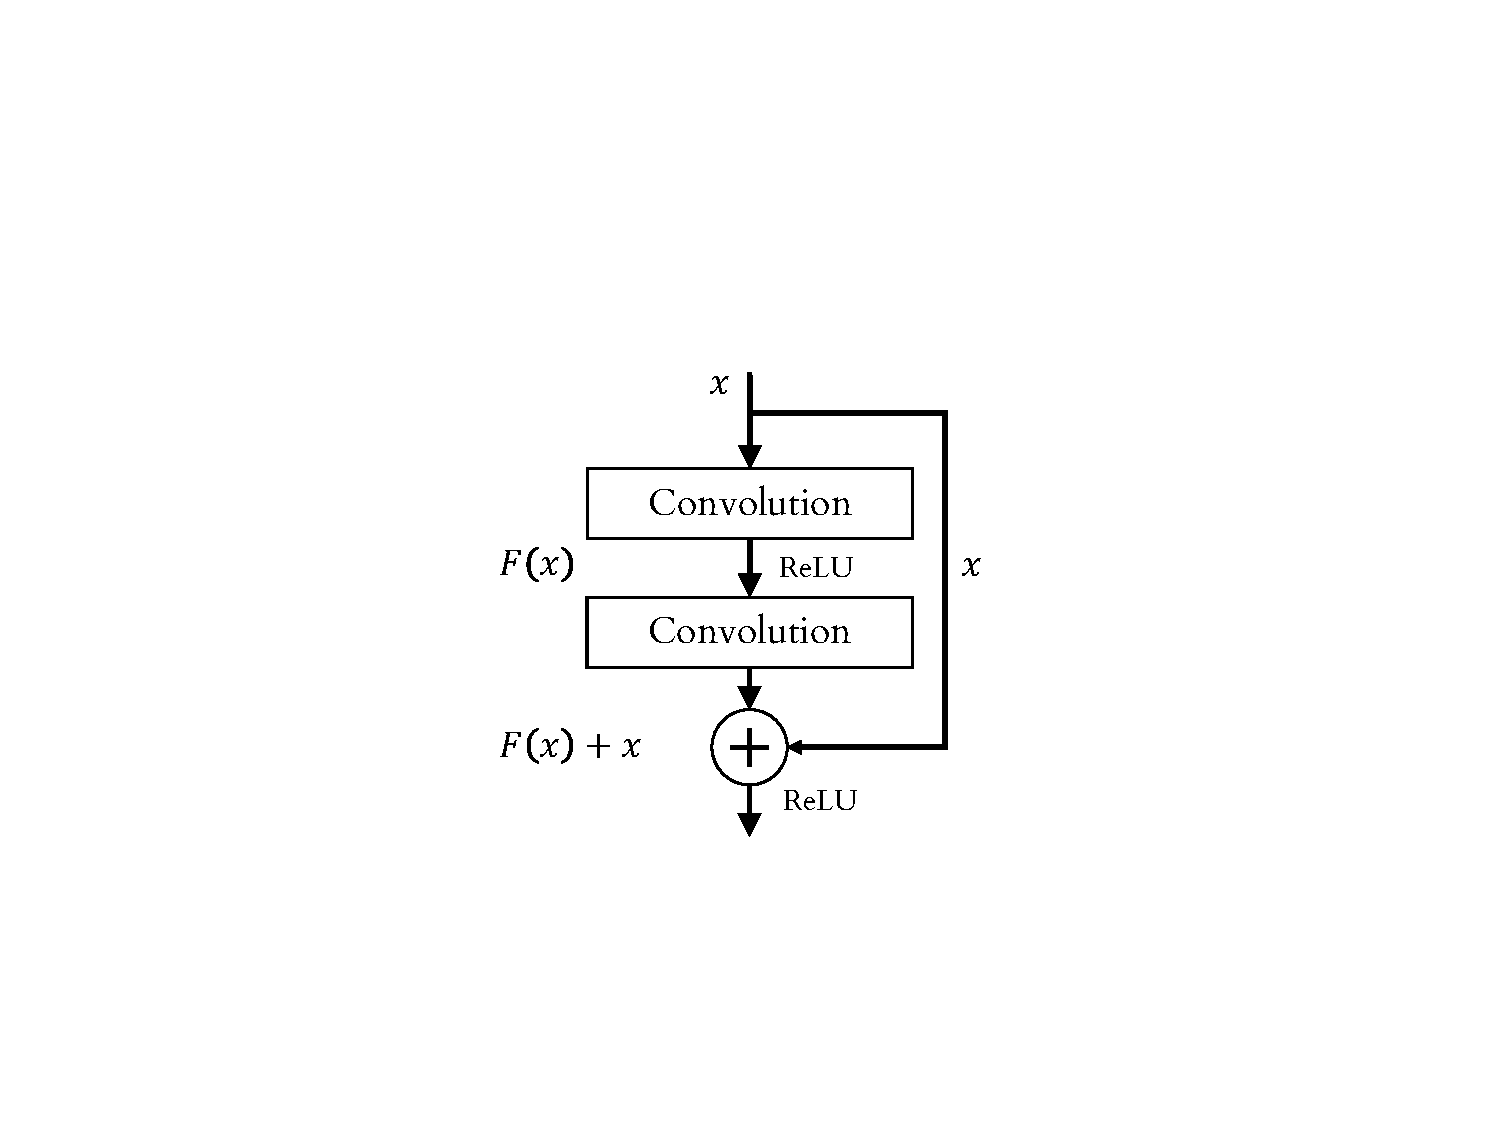
\includegraphics[width=0.45\textwidth, trim={7cm 4.8cm 7cm 6cm}, clip]{images/models/res_block}
  \caption{Schematic of a residual block with 2 convolutional layers.}
  \label{fig:res_block}
\end{figure}

Figure \ref{fig:res_block} shows an example residual block. The input to the block is fed into multiple subsequent convolutional layers with ReLU activation functions. The outputs of the last convolutional layer $F(x)$ are then added to the identity of the initial input $x$. This architecture allows the propagation of earlier features into later layers and helps avoid the problem of vanishing gradients that most predecessor architectures encountered \citep{alom_history_2018}. As a result, significantly deeper network designs can be created, most likely outperforming existing shallower architectures.

\begin{figure}[ht]
  \centering
  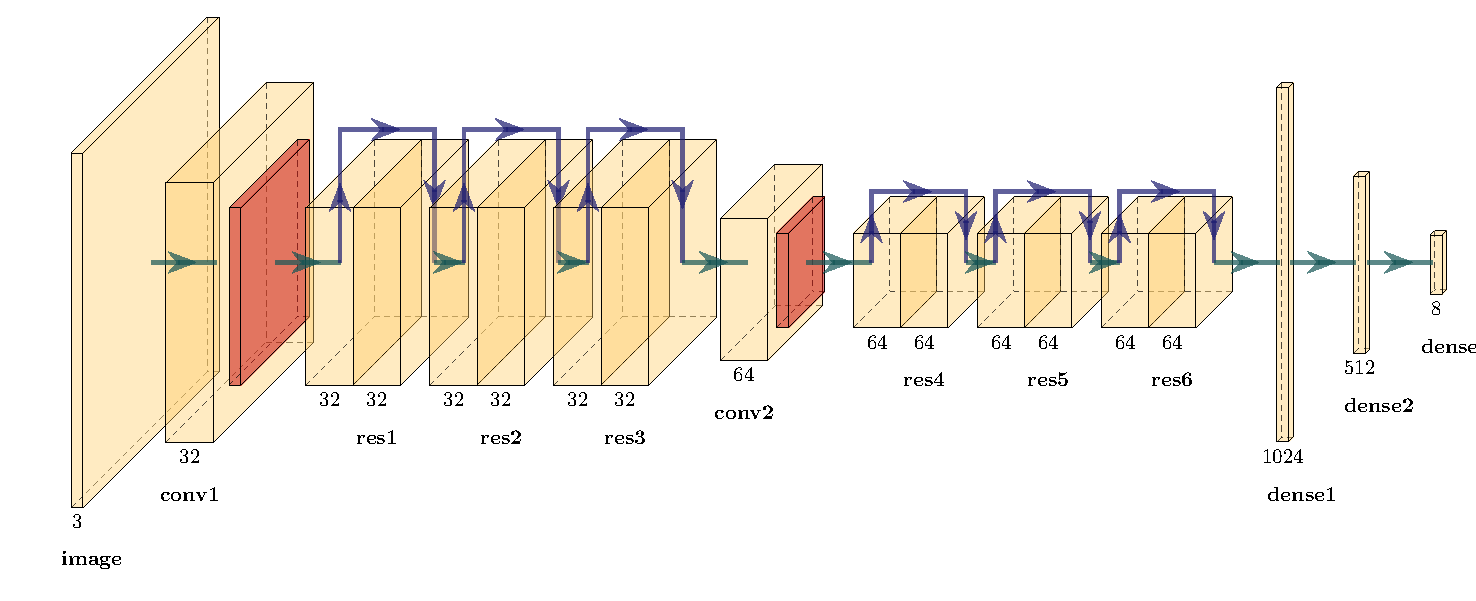
\includegraphics[width=0.9\textwidth]{images/models/resnet}
  \caption{Neural network architecture of the residual network.}
  \label{fig:resnet}
\end{figure}

The official paper proposes implementations of ResNet with 50, 101 and 152 layers. Since our dataset is significantly smaller than ImageNet, it is likely that these models would overfit on the training data without adding much benefit over a shallower architecture. Hence, we decided to implement our own version of ResNet with 6 residual blocks and a total of 14 convolutional layers. The architecture can be seen in Figure \ref{fig:resnet}.

The residual blocks are arranged in two groups of three. The convolutional kernels of each block have size $5 \times 5$. Each group of residual blocks is preceded by a single convolutional layer with a max pooling layer to reduce the input resolution. Similarly to AlexNet, we use two FC layers with dropout in the end, followed by a softmax-activated output layer. Despite the much deeper architecture compared to AlexNet, our ResNet implementation has only $4\,033\,160$ trainable parameters.

%----------------------------------------------------------------------------------------------------------------------------------


\section{Transfer learning using a pre-trained ResNet}
\label{transfer_learning}

An attempt was made to make use of transfer learning. We decided to evaluate an RGB-only, LWIR-only and feature fusion configuration of a pretrained network. 

Obtaining an RGB-only network with pretrained weights is easy. We used an implementation of ResNet 152 v2 \citep{he_identity_2016} with weights that were previously trained on the ImageNet dataset. Since ImageNet has 1000 classes, we had to replace the output layer of the network with our own custom layer, to make labels and outputs match.

As discussed in Section \ref{transfer_learning_analysis}, limited resources are available for transfer learning of thermal images. After some review, an annotated thermal dataset provided by FLIR was found \footnote{\url{https://www.flir.com/oem/adas/adas-dataset-form/}}. This dataset was deemed suitable because it was captured by another FLIR camera, minimising the sensor difference. Nonetheless, at $640 \times 512$, the thermal infrared resolution of the FLIR Tau 2 is significantly higher than that of the FLIR One Pro ($160 \times 120$) used for this project. The dataset contains a total of $10\,228$ frames with bounding box annotations for five classes: \textit{person}, \textit{car}, \textit{bicycle}, \textit{dog} and \textit{other vehicle}.

To use the bounding box annotations for our classification problem, we treated each bounding box as an individual sample, cropping the images appropriately. To reduce noise, we removed samples with a resolution below $40 \times 40$. Only thermal images were used. We then trained an off-the-shelf implementation of ResNet 50 v2 on this dataset. We chose this shallower version of ResNet due to the limited amount of available data and time. It was deemed unlikely that using a more complex, such as ResNet 152 v2 model would benefit performance significantly.

The feature fusion configuration of our transfer learning model, therefore, uses a ResNet 152 v2 for the RGB path, and a ResNet 52 v2 for the LWIR path.

%----------------------------------------------------------------------------------------------------------------------------------

\section{Mobile application design}

The mobile application was designed with two primary requirements in mind:

\begin{itemize}
  \item Enabling the easy capture of combined visible-light and thermal datasets.
  \item Being able to perform live multi-class classification on multiple species of animals.
\end{itemize}



%==================================================================================================================================
\chapter{Implementation}
\label{implementation}

\section{Frameworks and tools}

\subsection{Mobile application development}

The mobile application was developed using Android Studio and the Java programming language. To communicate with the FLIR sensor, we used the FLIR Thermal SDK for Android. A continuous delivery (CD) build pipeline was set up using GitHub Actions to verify that changes to the application do not include build-breaking bugs. To achieve this, the pipeline automatically downloads software dependencies, such as the FLIR SDK, compiles the application and provides a downloadable and installable APK file.

\subsection{Deep learning and image processing}

All neural networks were implemented using the TensorFlow deep learning framework \citep{abadi_TensorFlow_2016}. TensorFlow was chosen over alternatives such as PyTorch due to its built-in Keras API and due to its compatiblity with TensorFlow Lite. Keras is a high-level neural networks API that was developed by \citet{chollet_keras_2015} to enable fast experimentation. Keras was used in conjunction with other modules provided by the TensorFlow library. 

TensorFlow Lite is a set of tools aimed towards running deep learning models on mobile and internet of things (IoT) devices. It provides a Java API that can be used for Android application development and was, therefore, selected for the deployment of the model onto a mobile device.

To perform the various image processing tasks required for this project, we made use of scikit-image \citep{van_der_walt_scikit-image_2014} and the Python implementation of OpenCV \citep{bradski_opencv_2000}. Furthermore, the Java implementation of OpenCV was used for the Android application, making it possible to perform affine transformations on captured images on the edge device.

We computed the Grad-CAM visualisations of our networks using Keras-vis \citep{kotikalapudi_keras-vis_2017}.

\subsection{Hardware and environment}

Training a deep neural network is a time-consuming process. However, many of the operations that get executed when fitting and evaluating a deep learning model benefit from hardware-accelerated vectorised computation. Therefore, training and evaluation of a neural network can be several orders of magnitude faster on a GPU than on a CPU due to the GPU's ability for parallelised computations \citep{shi_benchmarking_2016}. 

Hence, Google Colaboratory (Colab) was used for the majority of the experimentation process and design of models. Colab is a cloud-hosted service that allows the execution of Jupyter Notebooks on free-to-use GPU runtimes. Therefore, we were able to leverage the power of a Nvidia Tesla P4 GPU with 8 GB of VRAM.

For more computationally expensive tasks, we made use of the GPU cluster provided by the faculty's Information, Data \& Analysis research section. The cluster provides access to nodes with more powerful resources than Colab, including 512 GB of RAM and multiple Nvidia GeForce RTX 2080 Ti GPUs with 24 GB of VRAM.

The cluster uses Openshift and the Kubernetes container management framework to assign resources to jobs. To be able to run computations on the cluster, we created a custom Docker image with all our software requirements, including TensorFlow and OpenCV. When scheduling a job, a container instance is created from this image that executes the supplied training script.

%----------------------------------------------------------------------------------------------------------------------------------

\section{Architecture and implementation details}

\subsection{Data loading}

Due to the limited amount of memory that Colab provides, it is impossible to pre-load the entire training dataset into memory for training. For this reason, a data loader class was implemented that supported lazy loading of data batches. When constructing the loader, a batch size can be specified, in addition to whether image samples shall be registered, and the target image resolution. 

Since the data loader extends Keras' \lstinline{Sequence} class, it fully integrates with the \lstinline{Model} training API. When constructed, it loads a list of all samples, containing image paths and class labels. It then enumerates the classes.

When \lstinline{model.fit()} is called with the data loader as data source, Keras will use the \lstinline{__getitem__()} function of the data loader repeatedly to lazily load batches of images into memory. The data loader will register images if specified and convert them into a tensor of shape $(batch\_size \times height \times width \times 4)$. Finally, it will return a tuple containing the image tensor and the one-hot representation of the numeric class labels.

While this approach was necessary to fit the model on the whole training dataset, we found that it noticably slowed down training speeds. This is most likely due to slow I/O bottlenecking the loading speed. Instead of having to load the dataset into memory once in the beginning, loading has to be performed for every training epoch. An attempt was made to use TensorFlow's data API instead of OpenCV for loading and pre-processing to load the data directly into VRAM. However, the performance improvement was negligible. Therefore, when running evaluations on the GPU cluster, we resorted to pre-loading all batches into memory, using our data loader class.

\subsection{Grid search}
\label{gridsearch_impl}

To evaluate the performance of the four different models and the six configurations, a grid search was run over all 24 possible combinations. For this purpose, we derived all models from a custom-built superclass \lstinline{AbstractModel}, to ensure that they implement a common API. This enabled us to iterate over all models and all configurations, training and evaluating every combination.

\subsection{Affine data augmentation}
\label{augmentation_impl}

Various tools are available to perform real-time data augmentation as part of the training pipeline. However, to achieve the highest possible level of control, a custom data augmentation function was designed. The function accepts a multiplication factor $n$ and leverages TensorFlow's \lstinline{ImageDataGenerator} to apply random affine transformations to images in the dataset.

The script works by counting the number of samples per class and determining the class with the highest support. Each sample in that class is then augmented $n$ times. Finally, all remaining classes are being augmented until their sample size reaches that of the max class. The aim of this algorithm is to provide an even dataset without class imbalances.


\subsection{Predicting LWIR images using an autoencoder}
\label{autoencoder_implementation}

\subsubsection{Traditional autoencoder}

A deep convolutional autoencoder was created to predict the LWIR signature of objects from the corresponding visible light image. The architecture of the network is shown in Figure \ref{fig:autoencoder_architecture}. The network consists of an encoder and a decoder that each contain four blocks of layers.

\begin{figure}[ht]
  \centering
  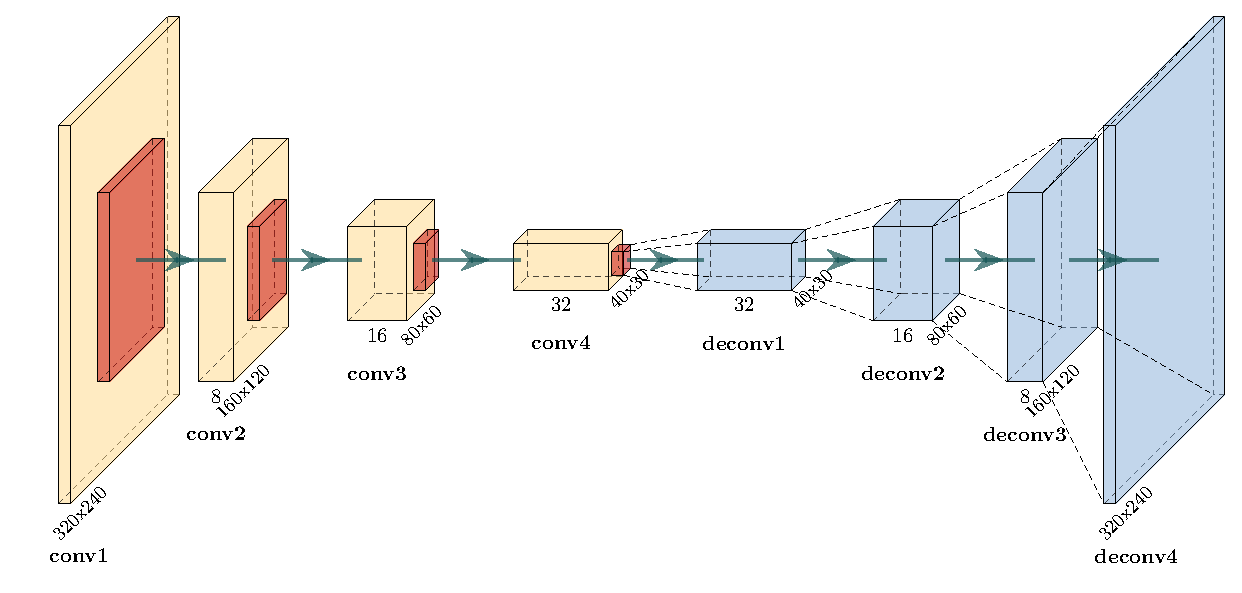
\includegraphics[width=0.9\textwidth]{images/models/autoencoder}
  \caption{Neural network architecture of the autoencoder.}
  \label{fig:autoencoder_architecture}
\end{figure}

Each encoder block has a convolutional layer, followed by a leaky ReLU activation function and a subsequent max pooling layer for downsampling. The $320 \times 240 \times 1$ input images are thus processed and downsampled to a $20 \times 15 \times 32$ tensor containing a compact, latent representation of the features in the original image.

The output of the decoder is then fed forward into four blocks of deconvolutional layers followed by leaky ReLU activation to attempt a reconstruction the LWIR image. Each deconvolutional layer tries to upsample the input by predicting appropriate pixel values.

Due to the lack of a discriminator, our autoencoder design does not satisfy the requirements of a generative adversarial network. However, autoencoders are commonly used for image processing tasks such as denoising and colorisation. As LWIR images are generally less noisy than visible light images (XXX proof) and both images share rough features such as edges, we deemed an autoencoder architecture to be appropriate for this generative task.

A subset of the animals training dataset with 415 images of Shetland ponies was chosen. Mean squared error was selected as the loss function. The network was trained for 100 epochs with a batch size of 16. Training time averaged around 18 minutes on an NVIDIA Tesla P-100 GPU.

\begin{figure}[ht]
  \centering
  \begin{subfigure}[h!]{0.22\textwidth}
    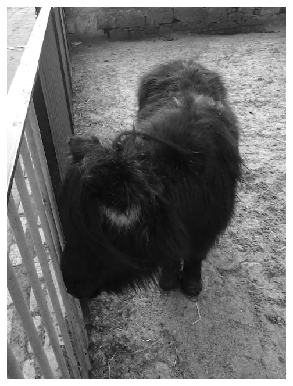
\includegraphics[width=\textwidth]{images/autoencoder/train/gray.png}
    \caption{Original image}
  \end{subfigure}
  \begin{subfigure}[h!]{0.22\textwidth}
    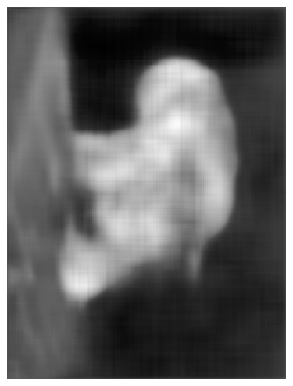
\includegraphics[width=\textwidth]{images/autoencoder/train/auto.png}
    \caption{Autoencoder prediction}
    \label{fig:autoencoder_pony_train_autoencoder}
  \end{subfigure}
  \begin{subfigure}[h!]{0.22\textwidth}
    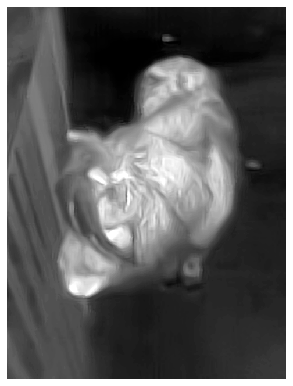
\includegraphics[width=\textwidth]{images/autoencoder/train/unet.png}
    \caption{U-Net prediction}
    \label{fig:autoencoder_pony_train_unet}
  \end{subfigure}
  \begin{subfigure}[h!]{0.22\textwidth}
    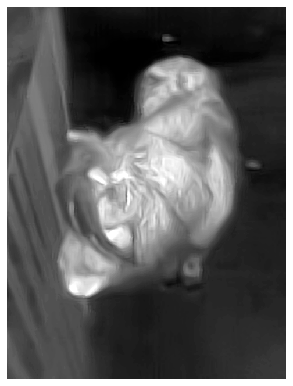
\includegraphics[width=\textwidth]{images/autoencoder/train/lwir.png}
    \caption{Actual LWIR image}
  \end{subfigure}
  \caption{Outputs of autoencoder and U-Net on training data.}
  \label{fig:autoencoder_pony_train}
\end{figure}

As can be seen in Figure \ref{fig:autoencoder_pony_train_autoencoder}, the network correctly identifies the pony from the training dataset and determines that it should have a higher local intensity in the LWIR waveband. However, when comparing the predicted to the actual LWIR image, it is apparent that the autoencoder lacks the ability to generate the fine textural details of the animal. This is very likely due to the denoising property caused by the encoder's bottleneck.

\subsubsection{U-Net}

U-Net was first introduced by \citet{ronneberger_u-net_2015} to improve performance of biomedical image segmentation systems. Similarly to a conventional autoencoder, it features a contracting path that downsamples or encodes the input, and a symmetric expanding path that upsamples or decodes the input. Additionally, for each deconvolutional layer, the output of the corresponding opposite convolutional layer is concatenated to the layer's input map. These connections can be seen in Figure \ref{fig:unet_architecture}, which visualises our custom U-Net implementation. 

\begin{figure}[ht]
  \centering
  \includegraphics[width=0.9\textwidth]{images/models/unet}
  \caption{Neural network architecture of the U-Net.}
  \label{fig:unet_architecture}
\end{figure}

We chose to evaluate this architecture because it combines the denoising features of a traditional autoencoder with the ability to generate finer textures due to its skip connections. Similar to the traditional autoencoder, the U-Net was trained for 100 epochs on the the same dataset. 

Figure \ref{fig:autoencoder_pony_train_unet} displays the predicted LWIR image for the pony from the training dataset. Unlike the autoencoder, the U-Net is able to accurately represent the texture of the animal in the LWIR waveband.

\subsubsection{Results on unknown data}

After successful training of the networks, two images of ponies were retrieved from Wikimedia Commons \footnote{\url{https://commons.wikimedia.org/wiki/File:Sandwick_Shetland_Pony.jpg}} \footnote{\url{https://commons.wikimedia.org/wiki/File:Shetland_ponies_at_Sandwick.jpg}}. They were then fed into the network in an attempt to generate the corresponding LWIR images. The respective outputs can be seen in Figure \ref{fig:autoencoder_pony}.

\begin{figure}[ht]
  \centering
  \begin{subfigure}[h!]{0.22\textwidth}
    \includegraphics[width=\textwidth]{images/autoencoder/pony_1/gray.png}
    \includegraphics[width=\textwidth]{images/autoencoder/pony_2/gray.png}
    \caption{Original images}
  \end{subfigure}
  \begin{subfigure}[h!]{0.22\textwidth}
    \includegraphics[width=\textwidth]{images/autoencoder/pony_1/auto.png}
    \includegraphics[width=\textwidth]{images/autoencoder/pony_2/auto.png}
    \caption{Autoencoder prediction}
  \end{subfigure}
  \begin{subfigure}[h!]{0.22\textwidth}
    \includegraphics[width=\textwidth]{images/autoencoder/pony_1/unet.png}
    \includegraphics[width=\textwidth]{images/autoencoder/pony_2/unet.png}
    \caption{U-Net prediction}
  \end{subfigure}
  \caption{Predicted LWIR signature of images of shetland ponies.}
  \label{fig:autoencoder_pony}
\end{figure}

It appears as if the traditional autoencoder is more successful at generating LWIR images with plausible shapes than the U-Net. Various artifacts can be spotted in the U-Net image. Overall, the shape of the pony is not accurately represented. It is likely that the U-Net is more likely to overfit on the training data.

Upon inspection of the bottom image, it can be seen that the white patch of the pony is also apparent in the autoencoder prediction. We conclude that the model is overfit on dark ponies and is, therefore, unable to detect the patch as a normal part of the animal. Nonetheless, it seems possible that the autoencoder prediction might be accurate enough to be able to generate additional training data for a classifier.

%----------------------------------------------------------------------------------------------------------------------------------


\section{Mobile application}

Figure \ref{fig:app_uml} shows the architecture of the mobile application. The required components were implemented in a modular, extendable framework. The \lstinline{MainActivity} displays a list of all discovered FLIR cameras, including emulators. Each list item is represented by an instance of \lstinline{CameraArrayAdapter} and allows the user to start a \lstinline{CameraActivity} or \lstinline{ClassifierActivity} for the given sensor. 

\begin{figure}[ht]
  \centering
  \includegraphics[width=0.8\textwidth, trim={2.5cm 4.5cm 2.5cm 4.5cm}, clip=true]{images/app/App_UML}
  \caption{Simplified UML class diagram of the mobile application.}
  \label{fig:app_uml}
\end{figure}

Both activities share common functionality by extending \lstinline{AbstractCameraActivity}. This includes the \lstinline{CameraHandler}, which is responsible for communicating with the FLIR device and receiving a stream of images from the sensor. Furthermore, the \lstinline{AffineTransformer} initialises the OpenCV backend and provides functionality to perform affine transformations on images.

The \lstinline{CameraActivity} is designed to enable users to capture multispectral datasets. It contains a button for starting and stopping a recording. In addition, it uses an instance of the \lstinline{ImageWriter} class to save the captured frames to device storage and add them to the gallery.

Finally, the \lstinline{ClassifierActivity} initialises an instance of \lstinline{ModelHandler}. This class loads the TensorFlow Lite model and the class labels and performs real-time predictions on the images provided by the \lstinline{CameraHandler}.



%==================================================================================================================================

\chapter{Evaluation}
\label{evaluation}

\section{Training strategies}

\subsection{Training-validation split}
\label{eval_train_val_split}

Multiple configurations of train/test split were attempted. Splitting the data with stratified sampling and train-validation-split of 80-20, the custom ResNet in fusion mode achieved perfect training and validation accuray, as can be seen in Figure \ref{fig:acc_stratified}.  

\begin{figure}[ht]
  \centering
  \begin{subfigure}[h!]{0.42\textwidth}
    \includegraphics[width=\textwidth, trim={0cm 0cm 0cm 0cm}, clip=true]{images/evaluation/stratified/accuracy}
    \caption{Accuracy over training epochs.}
    \label{fig:acc_stratified}
  \end{subfigure}
  \begin{subfigure}[h!]{0.4\textwidth}
    \includegraphics[width=\textwidth]{images/evaluation/stratified/heatmaps.png}
    \caption{Example class activation heatmaps.}
    \label{fig:heatmap_stratified}
  \end{subfigure}
  \caption{Evaluation results of the custom ResNet with stratified train-validation split.}
\end{figure}

This result is most likely due to the similarity of many images as mentioned in Section \ref{classes_samples}. Since training and validation samples are drawn from the same raw dataset, we conclude that it is very likely that the models are significantly overfitted on the captured data. It is unlikely that they would perform as well on chaotic new data as indicated by the validation accuracy. 

Figure \ref{fig:heatmap_stratified} shows two example class activation heatmaps for the trained model. In these two images, the focus of the classifier appears to be on many environmental features instead of the animals, supporting our theory.

Fitting the models on the training dataset as defined in Section \ref{classes_samples}, validation scores dropped significantly. This was in accordance with our expectations, as the samples from the training and validation datasets are mostly independent. Therefore, the models are not able to overfit on the whole dataset anymore and the validation score is more representative of potential performance on new data.

\subsection{Data augmentation}

\subsubsection{Affine transformation}

The data augmentation strategy as described in Section \ref{augmentation_impl} was evaluated by applying the augmentation script to the training dataset twice, with a factor of 2 and 5 respectively. The augmented datasets, thus, contain around 2 and 5 times as many samples than the original dataset. Furthermore, the class imbalances have been equalised by the script by creating more samples of the underrepresented classes.

The custom ResNet in fusion mode was trained on the original and the two augmented datasets for 80 epochs. The complete classification reports can be inspected in Appendix \ref{appendix_augmentation_affine}. The overall f1-score increased from $0.73$ without any augmentation to $0.78$ with augmentation with a factor of 2. For the factor-5-dataset, a slight increase of the f1-score to $0.79$ was determined.

\subsubsection{Generation of artificial data}

We used the autoencoder from Section \ref{autoencoder_implementation} to predict the LWIR signatures of ten images retrieved from Wikimedia Commons (Appendix \ref{appendix_augmentation}). We then selected a subset of our training dataset, containing images of the \textit{pony}, \textit{alpaca} and \textit{chicken} classes. A second copy of this dataset was created and the ten predicted images were appended to the \textit{pony} class.

The custom ResNet in late feature-fusion configuration was trained on both datasets. The full classification scores can be inspected in Appendices \ref{table:auto_scores_normal} and \ref{table:auto_scores_auto}. 

\begin{figure}[ht]
  \centering
  \begin{subfigure}[h!]{0.3\textwidth}
    \includegraphics[width=\textwidth]{images/evaluation/autoencoder/confusion_normal}
    \caption{Without generated images.}
    \label{fig:auto_confusion_normal}
  \end{subfigure}
  \begin{subfigure}[h!]{0.3\textwidth}
    \includegraphics[width=\textwidth]{images/evaluation/autoencoder/confusion_autoencoder}
    \caption{With generated images.}
    \label{fig:auto_confusion_auto}
  \end{subfigure}
  \caption{Confusion matrix of the custom ResNet in late feature-fusion configuration on a simplified training dataset including and excluding artificially generated samples.}
  \label{fig:auto_confusion}
\end{figure}

The confusion matrices in Figure \ref{fig:auto_confusion} show that the amount of correctly classified ponies has indeed increased after including the artificially generated samples. However, more chicken and alpacas are mistakenly classified as ponies. In numbers, the recall of the \textit{pony} class improved from $0.80$ to $0.87$, while the precision dropped from $0.73$ to $0.69$. The weighted average f1-score across the dataset remains unchanged at $0.82$.

%----------------------------------------------------------------------------------------------------------------------------------

\section{Hyperparameters}


\subsection{Network architecture and configuration}

To determine the configuration with the best performance out of all proposed models, we ran a grid search as described in Section \ref{gridsearch_impl}. All models were trained for 80 epochs with a batch size of 32 samples. We chose Adam as the optimiser with a learning rate of $10^{-6}$. 

The complete loss and accuracy history of all models and configurations are shown in Appendix \ref{appendix_grid_search}. Overall, the custom CNN yielded the lowest performance out of the three models. This is unsurprising, given the small number of trainable parameters compared to the other two models.

\begin{figure}[ht]
  \centering
  \includegraphics[width=0.8\textwidth]{images/evaluation/gridsearch/ResNet}
  \caption{Training and validation loss and accuracy of different configurations of the ResNet implementation.}
  \label{fig:resnet_configs}
\end{figure}

Out of the three models, our ResNet implementation performed best. The results for this model can be seen in Figure \ref{fig:resnet_configs}. For all configurations some overfitting can be observed, as the training losses and accuracies converge at near perfect values.

The LWIR-only configuration appears to be the least effective overall. 

(XXX)

Among all configurations, the late feature fusion model achieved the highest accuracy. Furthermore, cross-entropy loss is comparatively low. This result confirms our theory that late feature fusion based approach proposed by \citet{wagner_multispectral_2016} can be applied to our multi-class classification problem. Thus, we selected this configuration as our final classifier. 

\subsection{Batch size}

(XXX TODO: REWORK NEEDED)

An influential hyperparameter for training neural networks is batch size \citep{ioffe_batch_2015}. The batch size during training determines how many samples are used for each optimisation step. Generally, smaller batch sizes result in the training loss converging in fewer epochs, while larger batch sizes offer better computational efficiency due to parallelisability \cite{devarakonda_adabatch_2018}.

Furthermore, smaller batch sizes make the training process more stochastic. More steps are taken during training. However, the lower amount of samples per batch means that steps are less likely to be in the direction of the global minimum. On the other hand, it is more likely that the model can avoid getting stuck in local minima. \citet{smith_dont_2018} state that increasing the batch size can help the optimisation algorithm converge on the global minimum, instead of bouncing around the optimum. \citet{radiuk_impact_2017} conclude that SGD performs better with larger batch sizes on the MNIST and CIFAR-10 datasets.

To evaluate the effect of different batch sizes on the validation accuracy of our model, we trained our implementation of ResNet in fusion configuration with batch sizes of 2, 8, 32, and 128. We chose the Adam optimizer with an initial learning rate of $10^{-6}$. The results can be seen in Figure \ref{fig:batch_size}.

\begin{figure}[ht]
  \centering
  \includegraphics[width=0.8\textwidth]{images/evaluation/batch_size/history}
  \caption{Training and validation loss and accuracy with varying batch sizes.}
  \label{fig:batch_size}
\end{figure}

As expected, when training with smaller batch sizes, we can observe a much faster convergence of loss and accuracy. Furthermore, the validation accuracy with the lower batch sizes appears to be higher than that of larger batch sizes. However, lower batch sizes also have a larger validation loss. This can be an indicator for overfitting. Accuracy is a discrete measure, whereas cross-entropy takes probabilities and confidence into consideration.

%----------------------------------------------------------------------------------------------------------------------------------

\section{Final classifier}

To obtain reliable scores for the selected model, we ran a 10-fold cross validation on the late feature fusion ResNet and averaged the results. Since the validation dataset had to be kept completely separate from the training dataset as a result of Section \ref{eval_train_val_split}, the k-fold split was performed only on the training dataset. During each fold, the non-selected samples were discarded instead of being used for validation.

Table \ref{table:final_classifier_scores} shows the precision, recall and f1-score of each class. The classes with the highest f1-score are \textit{goose}, \textit{cat} and \textit{hamburg chicken}. The classes with the lowest f1-score are and \textit{pony} and \textit{muscovy duck}. The pony class stands out with particularly low recall. Only half of all pony samples were classified correctly.

\begin{table}[ht]
  \centering
  \begin{tabular}{@{}lllll@{}}
  \toprule
                        & \textbf{precision} & \textbf{recall} & \textbf{f1-score} &  \\ \midrule
  Cat                   & 0.87               & 1.00            & 0.93              &  \\
  Pony                  & 0.74               & 0.49            & 0.59              &  \\
  Hamburg chicken       & 0.91               & 0.88            & 0.90              &  \\
  Alpaca                & 0.98               & 0.67            & 0.79              &  \\
  Muscovy Duck          & 0.57               & 0.86            & 0.69              &  \\
  Chicken               & 0.64               & 0.85            & 0.73              &  \\
  Silkie Chicken        & 1.00               & 0.59            & 0.74              &  \\
  Goose                 & 0.96               & 1.00            & 0.98              &  \\
  \midrule
  \textbf{Weighted avg} & \textbf{0.83}      & \textbf{0.80}   & \textbf{0.80}     &  \\ \bottomrule
  \end{tabular}
  \caption{Precision, recall and f1-score of the final late feature fusion ResNet model.}
  \label{table:final_classifier_scores}
\end{table}

The chicken and muscovy duck classes suffer especially from low precision. This means that many samples are wrongly classified as those classes. A possible explanation for this is the high variety of environments within the chicken and muscovy duck datasets. As outlined in Table \ref{table:train_test_dataset}, the amount of subsets used for the training dataset is very high for both classes. It is possible that the model is biased in favour of these  classes due to the high variety of backgrounds.


\subsection{t-SNE}
\label{tsne}

To further analyse these findings, we made use of t-distributed stochastic neighbour embedding (t-SNE), which was first introduced by \citet{maaten_visualizing_2008}. t-SNE is a dimensionality reduction technique for the visualisation of high-dimensional data. By flattening each image into a single vector, we obtain high-dimensional data points that t-SNE can be applied to. The result is a 2-D representation of the images that can be easily plotted and inspected. The same process can be applied to the outputs of the layers of the neural network.

Figure \ref{fig:test_tsne} shows the result of applying t-SNE to the validation dataset. In all four visualisations, most samples are concentrated in small clusters. These clusters most likely correspond to the subsets of the validation dataset. Images that were captured in quick temporal succession are likely to be very similar, which is why they are very close together in the t-SNE visualisation. Figure \ref{fig:test_tsne_fc} demonstrates that, overall, the network successfully seperates the samples into distinct classes.

\begin{figure}[ht]
  \centering
  \begin{subfigure}[h!]{0.4\textwidth}
    \includegraphics[width=\textwidth, trim={1cm 1cm 1cm 1cm}, clip]{images/evaluation/embedding/val/input}
    \caption{Input image.}
    \label{fig:test_tsne_input}
  \end{subfigure}
  \quad
  \begin{subfigure}[h!]{0.4\textwidth}
    \includegraphics[width=\textwidth, trim={1cm 1cm 1cm 1cm}, clip]{images/evaluation/embedding/val/vis}
    \caption{Output of final conv layer of VIS branch.}
    \label{fig:test_tsne_vis}
  \end{subfigure}

  \begin{subfigure}[h!]{0.4\textwidth}
    \includegraphics[width=\textwidth, trim={1cm 1cm 1cm 1cm}, clip]{images/evaluation/embedding/val/lwir}
    \caption{Output of final conv layer of LWIR branch.}
    \label{fig:test_tsne_lwir}
  \end{subfigure}
  \quad
  \begin{subfigure}[h!]{0.4\textwidth}
    \includegraphics[width=\textwidth, trim={1cm 1cm 1cm 1cm}, clip]{images/evaluation/embedding/val/fc}
    \caption{Output of final fully-connected layer.}
    \label{fig:test_tsne_fc}
  \end{subfigure}
  \caption{t-SNE visualisation of the validation dataset. As the features progress through the layers of the neural network, the classes become more easily separable.}
  \label{fig:test_tsne}
\end{figure}

As can be seen in Figure \ref{fig:test_tsne_input}, the cat images clearly stand out from the other classes even before being fed into the model. This is most likely a result of the fact that the cat images are the only ones that were captured in an indoor setting, resulting in a significantly lower illumination level.

This interpretation is further supported by the observation that the strict separation of the cat cluster persists throughout the VIS branch of the network, as shown in \ref{fig:test_tsne_vis}. The LWIR band, however, is not sensitive to illumination. Therefore, the LWIR branch of the network is unable to use the overall brightness of the image to make inferences about the classes. This explains why the distinctive cat cluster is not visible in Figure \ref{fig:test_tsne_lwir}.

A similar effect can be observed for the hamburg chicken class. Unlike for the cat class, a large hamburg chicken cluster stands out in the t-SNE of the input image as well as the final convolutional layers of the VIS and LWIR branches. A likely explanation for this pheonomenon is that many images of hamburg chicken are partly occluded by a grid. Since this is unique to this class, it can be assumed that the model uses the grid as a feature to identify hamburg chicken, resulting in undesirable overfitting on the environment.


\subsection{Saliency analysis}

Saliency maps were first introduced by \citet{itti_model_1998} as a means of representing the conspicuity of every spatial location in an image. \citet{simonyan_deep_2014} developed this concept into class-specific saliency maps by using back-propagation of a classification.

Gradient-weighted Class Activation Mapping (Grad-CAM) is a novel visualisation technique developed by \citet{selvaraju_grad-cam_2020}. It uses the gradients of a target class at the last convolutional layer of a network to generate a heatmap showing the most important regions for the classification of that class.

Since the late feature fusion configuration of our ResNet has two parallel final convolutional layers, the gradient has to be computed for both layers. Figure \ref{fig:grad_cam} displays the Grad-CAM visualisation of four example images.

\begin{figure}[ht]
  \centering
  \begin{subfigure}[h!]{0.45\textwidth}
    \includegraphics[width=\textwidth]{images/evaluation/grad_cam/pos}
    \caption{Desirable example for both channels.}
    \label{fig:grad_cam_pos}
  \end{subfigure}
  \quad
  \begin{subfigure}[h!]{0.45\textwidth}
    \includegraphics[width=\textwidth]{images/evaluation/grad_cam/neg}
    \caption{Undesirable example for both channels.}
    \label{fig:grad_cam_neg}
  \end{subfigure}

  \begin{subfigure}[h!]{0.45\textwidth}
    \includegraphics[width=\textwidth]{images/evaluation/grad_cam/vis}
    \caption{Desirable VIS example.}
    \label{fig:grad_cam_vis}
  \end{subfigure}
  \quad
  \begin{subfigure}[h!]{0.45\textwidth}
    \includegraphics[width=\textwidth]{images/evaluation/grad_cam/lwir}
    \caption{Desirable LWIR example.}
    \label{fig:grad_cam_lwir}
  \end{subfigure}
  \caption{Grad-CAM visualisation of four example images. Warmer colours correspond to more attention by the last convolutional layer of the network. The left images are the VIS images and corresponding heatmaps. The LWIR image and heatmap can be seen in the right images.}
  \label{fig:grad_cam}
\end{figure}

Figure \ref{fig:grad_cam_pos} shows a desirable example. Both final convolutional layers of the network focus on the head and feet of the alpaca to identify the class. This implies high generalisability even for images in different environments.

However, the network does not always focus on the desired relevant parts of the images. In the example shown in Figure \ref{fig:grad_cam_neg}, both the VIS and LWIR branches of the network do not focus on the muscovy duck. Instead, attention is directed towards the environment, such as the grass texture. It is unlikely that the network will be able to predict similar images with a different background.

The remaining two subfigures display examples where only either the VIS or LWIR branches of the network focus on the animals. These cases demonstrate an advantage of the multi-branch approach. The network performs better overall, as it can rely on the features of two semi-redundant branches.


\subsection{Accuracy at different lighting conditions}

As discussed in Section \ref{modality}, the modality difference between VIS and LWIR images suggests that thermal imaging systems should perform better in low-light conditions compared to visible-light-only systems.

To evaluate the relationship between classification performance and illumination, we calculated the mean and standard deviation of all pixel values of each image in the validation dataset. We then determined the cross entropy loss of each prediction by the VIS-only, LWIR-only and late feature-fusion ResNets and plotted it as a function of mean and standard deviation. The results are shown in Figure \ref{fig:illumination}.

\begin{figure}[ht]
  \centering
  \includegraphics[width=0.8\textwidth]{images/evaluation/illumination}
  \caption{Cross entropy loss as a function of intensity mean and std of VIS and LWIR images in the validation dataset. The data has been smoothened with a running mean to show general trends.}
  \label{fig:illumination}
\end{figure}

The overall result defies the expected behaviour of the models. It can be seen that the LWIR-only network performs significantly worse than its VIS-only and late feature fusion counterparts on low-light images. This further supports the theory we formulated in Section \ref{tsne}. The LWIR-only network likely uses the darkness of the cat images as a biased feature of the cat class, giving it near perfect performance.

Since the LWIR band is not sensitive to illumination, the cat pictures do not generally stand out compared to in the VIS images. To obtain more robust results, a dataset with more well-balanced illumination levels would have to be acquired.

Furthermore, the LWIR-only network has a high loss on samples with low LWIR mean intensity. A possible explanation for this is the lack of visible features in these images. 

\subsection{Comparison against the baseline}

As shown in Figure \ref{fig:resnet_configs}, the final late feature-fusion model outperforms the visible-light-only baseline. It converges after around 50 epochs and remains fairly stable. The final f1-score of $80\%$ is a significant improvement over the $74\%$ achieved by the VIS-only network. We, therefore, conclude that this architecture yields a tangible benefit to our computer vision system.

To put these results into a relevant context, we compared the final classifier to a second, state-of-the-art baseline. This model, as described in \ref{transfer_learning}, is an instance of ResNet152 v2 that has been pre-trained on the ImageNet dataset and transfer-trained on our dataset.

The full training history is shown in Appendix \ref{appendix_baseline} (XXX insert). The VIS-only classifier achieved a final f1-score of $89\%$, significantly outperforming our best model. Our attempts to create a pre-trained late feature fusion model using the ImageNet data for the VIS branch and the FLIR dataset for the LWIR branch did not improve this baseline (XXX insert final score).

Since larger training datasets usually result in more generalisable models and ImageNet contains over a million annotated samples, this result is unsurprising. As a consequence of the aforementioned increased performance of the multispectral model compared to the VIS-only variant, we deem it likely that the pre-traiend baseline could be beat given a large enough dataset.


%----------------------------------------------------------------------------------------------------------------------------------

\section{Mobile application deployment}

\subsection{Functionality validation}

To verify whether the deployment of the model to the mobile application is functional, a live evaluation on the actual animals was planned. The intention was to point the phone with the FLIR camera at the objects to evaluate the quality of the predictions. Since unforseen circumstances emerged as a result of the SARS-CoV-2 epidemic, this evaluation could not be performed.

Instead, we qualitatively evaluated the deployment of the final model by pointing the phone and sensor at pictures from the existing validation dataset. Figure \ref{fig:app_screenshots} shows screenshots of the mobile application during this evaluation. A sample image was drawn from each class. Out of all eight images, the app gave six correct predictions.

It can, therefore, be concluded that the model is working correctly in the mobile application. Due to the physical limitations of the evaluation, the thermal channel could not be taken into consideration by the model, making the predictions less accurate. Furthermore, we observed a strong fluctuation of the predicted probabilities over time.

\begin{figure}[ht]
  \centering
  \begin{subfigure}[h!]{0.3\textwidth}
    \includegraphics[width=\textwidth]{images/app/screenshot_0.jpg}
  \end{subfigure}
  \begin{subfigure}[h!]{0.3\textwidth}
    \includegraphics[width=\textwidth]{images/app/screenshot_1.jpg}
  \end{subfigure}
  \begin{subfigure}[h!]{0.3\textwidth}
    \includegraphics[width=\textwidth]{images/app/screenshot_2.jpg}
  \end{subfigure}
  \caption{Screenshots of the mobile application's predictions with the feature-fusion model. Due to exceptional circumstances, only pictures of animals could be evaluated instead of the animals themselves.}
  \label{fig:app_screenshots}
\end{figure}

\subsection{Performance and latency}

The application was installed on a OnePlus 7 Android device to evaluate the latency of real-time classification. TensorFlow Lite was configured to use the device's GPU for predictions to guarantee the best possible performance. The RGB-only and feature-level fusion configurations of the custom ResNet were evaluated by running the application in classification mode and performing 1000 predictions. The application displays the mean and standard deviation of classification times since launch. 

Whereas the RGB-only model took an average of $40.99 ms$, $\sigma = 4.55 ms$ for a single prediction, the feature-fusion model performed a prediction every $70.24 ms$, $\sigma = 6.79 ms$. This equates to $14.24$ predictions per second, which is significantly higher than the sensor frame rate of $8.7 Hz$. Thus, we conclude that the the multispectral model is suitable for real-time classification tasks on edge devices.

%----------------------------------------------------------------------------------------------------------------------------------

\section{Issues and caveats}

\begin{enumerate}
  \item Cross-validation
  \item Better dataset
  \item GAN
  \item Evaluation of low-light scenarios
\end{enumerate}

%==================================================================================================================================
\chapter{Conclusion}

\section{Summary}

This dissertation explored the benefits and drawbacks of multispectral image classification with a thermal and visible light camera. A classifier based on the ResNet deep learning architecture was developed, achieving a validation f1-score of $80\%$.

Our evaluation demonstrates that a model based on late feature-level fusion of the thermal and visible light features, similar to \citet{wagner_multispectral_2016} clearly outperforms the VIS-only baseline. This is the case even in settings with sufficient illumination.

The classifier has been successfully deployed to a mobile edge device and can be run in real-time with tolerable latency. This demonstrates the suitability of the system for mobile environments with low computational power, such as phones and self-driving cars.

However, our model was not able to beat the second proposed baseline of a state-of-the art VIS-only classifier that was pre-trained on the ImageNet dataset. Attempts to perform transfer learning on an LWIR classifier did not manage to improve our model's performance. We conclude that the lack of available thermal datasets remains a signficant problem for the development of LWIR-based computer vision systems.

Furthermore, our t-SNE and saliency analysis of the final model reveals problems with bias and overfitting on the environment. These issues are likely a result of a noisy and insufficiently diverse dataset.

Nonetheless, our evaluation suggests that our multi-branch network architecture increases the system's robustness by providing more redundant features (XXX rephrase). We conclude that thermal multispectral imaging can significantly improve the performance of deep learning models for the recognition of animals.

%----------------------------------------------------------------------------------------------------------------------------------

\section{Future work}

We attempted to increase the generalisability of our classifier by generating artificial LWIR data using a convolutional autoencoder. Since the scale of this experiment was limited, no reliable conclusion about the effectiveness of this strategy could be drawn. To further evaluate the feasability of incorporating artifically generated data into the training process, a generative adversarial network could be designed and applied to a sufficiently large visible light dataset.

Moreover, many generalisation problems of our model are likely a result of poorly framed input images. Furthermore, the framing of objects is likely to be noisy when using the mobile application. A more robust approach for this usage scenario could involve the development of an object detection model. Such a model would support the detection of multiple objects in a single image at varying distances and positions. State-of-the-art architectures such as YOLO \citep{redmon_you_2016, redmon_yolov3_2018} promise low inference times and might be suitable for this task. 

Finally, for applications with stationary systems such as intruder detection or wildlife tracking, a model (XXX).

%==================================================================================================================================
%
% 
%==================================================================================================================================
%  APPENDICES  

\begin{appendices}

%==================================================================================================================================

\chapter{Multispectral CNN configurations}
\label{appendix_arch}

\begin{figure}[ht]
  \centering
  \includegraphics[width=0.25\textwidth]{images/models/keras/stacked.png}
  \caption{Architecture of AlexNet in stacked configuration.}
\end{figure}

\begin{figure}[ht]
  \centering
  \includegraphics[width=0.6\textwidth]{images/models/keras/voting.png}
  \caption{Architecture of AlexNet in voting configuration.}
\end{figure}

\begin{figure}[ht]
  \centering
  \includegraphics[width=0.6\textwidth]{images/models/keras/fusion.png}
  \caption{Architecture of AlexNet in late feature fusion configuration.}
\end{figure}

%==================================================================================================================================

\chapter{Data augmentation evaluation}
\label{appendix_augmentation}

\section{Affine transformation}
\label{appendix_augmentation_affine}

\begin{table}[H]
  \centering
  \begin{tabular}{@{}lllll@{}}
  \toprule
                        & \textbf{precision} & \textbf{recall} & \textbf{f1-score} &  \\ \midrule
  Cat                   & 0.57               & 1.00            & 0.72              &  \\
  Pony                  & 0.83               & 0.60            & 0.70              &  \\
  Hamburg chicken       & 0.74               & 0.89            & 0.81              &  \\
  Alpaca                & 1.00               & 0.52            & 0.68              &  \\
  Muscovy Duck          & 0.59               & 0.65            & 0.62              &  \\
  Chicken               & 0.53               & 0.61            & 0.57              &  \\
  Silkie Chicken        & 1.00               & 0.60            & 0.75              &  \\
  Goose                 & 0.98               & 1.00            & 0.99              &  \\
  \midrule
  \textbf{Weighted avg} & \textbf{0.78}      & \textbf{0.73}   & \textbf{0.73}     &  \\ \bottomrule
  \end{tabular}
  \caption{Precision, recall and f1-score of the late feature fusion ResNet model without affine data augmentation.}
  \label{table:appendix_affine_1}
\end{table}

\begin{table}[H]
  \centering
  \begin{tabular}{@{}lllll@{}}
  \toprule
                        & \textbf{precision} & \textbf{recall} & \textbf{f1-score} &  \\ \midrule
  Cat                   & 0.70               & 1.00            & 0.82              &  \\
  Pony                  & 0.97               & 0.59            & 0.73              &  \\
  Hamburg chicken       & 0.96               & 0.86            & 0.91              &  \\
  Alpaca                & 1.00               & 0.63            & 0.77              &  \\
  Muscovy Duck          & 0.53               & 0.86            & 0.65              &  \\
  Chicken               & 0.61               & 0.74            & 0.67              &  \\
  Silkie Chicken        & 1.00               & 0.57            & 0.73              &  \\
  Goose                 & 1.00               & 1.00            & 1.00              &  \\
  \midrule
  \textbf{Weighted avg} & \textbf{0.84}      & \textbf{0.78}   & \textbf{0.78}     &  \\ \bottomrule
  \end{tabular}
  \caption{Precision, recall and f1-score of the late feature fusion ResNet model with affine data augmentation (factor 2).}
  \label{table:appendix_affine_2}
\end{table}

\begin{table}[H]
  \centering
  \begin{tabular}{@{}lllll@{}}
  \toprule
                        & \textbf{precision} & \textbf{recall} & \textbf{f1-score} &  \\ \midrule
  Cat                   & 0.89               & 1.00            & 0.94              &  \\
  Pony                  & 0.97               & 0.48            & 0.64              &  \\
  Hamburg chicken       & 1.00               & 0.79            & 0.88              &  \\
  Alpaca                & 0.97               & 0.74            & 0.84              &  \\
  Muscovy Duck          & 0.47               & 0.78            & 0.59              &  \\
  Chicken               & 0.61               & 0.84            & 0.70              &  \\
  Silkie Chicken        & 1.00               & 0.57            & 0.73              &  \\
  Goose                 & 1.00               & 1.00            & 1.00              &  \\
  \midrule
  \textbf{Weighted avg} & \textbf{0.85}      & \textbf{0.79}   & \textbf{0.79}     &  \\ \bottomrule
  \end{tabular}
  \caption{Precision, recall and f1-score of the late feature fusion ResNet model with affine data augmentation (factor 5).}
  \label{table:appendix_affine_3}
\end{table}

%----------------------------------------------------------------------------------------------------------------------------------

\section{Artificial data}

\begin{captionedList}
  \begin{enumerate}
    \item{\url{https://commons.wikimedia.org/wiki/File:Shetland_pony_in_the_snow,_Baltasound_-_geograph.org.uk_-_1691743.jpg}}
    \item{\url{https://commons.wikimedia.org/wiki/File:Sandwick_Shetland_Pony.jpg}}
    \item{\url{https://commons.wikimedia.org/wiki/File:Shetland_pony_(2).jpg}}
    \item{\url{https://commons.wikimedia.org/wiki/File:Grey_Shetland_pony_-_geograph.org.uk_-_1606748.jpg}}
    \item{\url{https://commons.wikimedia.org/wiki/File:Shetland_Ponies_and_Iron_Horse,_Huxter,_Whalsay,_Shetland_-_geograph.org.uk_-_145763.jpg}}
    \item{\url{https://commons.wikimedia.org/wiki/File:Shetland_ponies_at_Sandwick.jpg}}
    \item{\url{https://commons.wikimedia.org/wiki/File:Pony_at_Mosedale.jpg}}
    \item{\url{https://commons.wikimedia.org/wiki/File:Pony_on_Lund_beach_-_geograph.org.uk_-_1741711.jpg}}
    \item{\url{https://commons.wikimedia.org/wiki/File:Fell_ponies,_West_Fell.jpg}}
    \item{\url{https://commons.wikimedia.org/w/index.php?title=Special:Search&limit=20&offset=420&profile=default&search=shetland+pony&advancedSearch-current=%7B%7D&ns0=1&ns6=1&ns12=1&ns14=1&ns100=1&ns106=1#/media/File:Jielbeaumadier_cheval_5_scva_paris_2012.jpeg}}
  \end{enumerate}
  \caption{Image sources for the autoencoder. All images retrieved under the Creative Commons licence.}
\end{captionedList}

\begin{table}[H]
  \centering
  \begin{tabular}{@{}lllll@{}}
  \toprule
                        & \textbf{precision} & \textbf{recall} & \textbf{f1-score} &  \\ \midrule
  Pony                  & 0.73               & 0.80            & 0.77              &  \\
  Alpaca                & 1.00               & 0.60            & 0.75              &  \\
  Chicken               & 0.80               & 0.99            & 0.89              &  \\
  \midrule
  \textbf{Weighted avg} & \textbf{0.85}      & \textbf{0.82}   & \textbf{0.82}     &  \\ \bottomrule
  \end{tabular}
  \caption{Precision, recall and f1-score of the custom ResNet in late feature fusion configuration on the simplified dataset including artificially generated samples.}
  \label{table:auto_scores_normal}
\end{table}

\begin{table}[H]
  \centering
  \begin{tabular}{@{}lllll@{}}
  \toprule
                        & \textbf{precision} & \textbf{recall} & \textbf{f1-score} &  \\ \midrule
  Pony                  & 0.69               & 0.87            & 0.77              &  \\
  Alpaca                & 1.00               & 0.60            & 0.75              &  \\
  Chicken               & 0.84               & 0.97            & 0.90              &  \\
  \midrule
  \textbf{Weighted avg} & \textbf{0.86}      & \textbf{0.83}   & \textbf{0.82}     &  \\ \bottomrule
  \end{tabular}
  \caption{Precision, recall and f1-score of the custom ResNet in late feature fusion configuration on the simplified dataset including artificially generated samples.}
  \label{table:auto_scores_auto}
\end{table}

%==================================================================================================================================

\chapter{Grid search results}
\label{appendix_grid_search}

\begin{figure}[ht]
  \centering
  \includegraphics[width=0.6\textwidth]{images/evaluation/gridsearch/comparison}
  \caption{Validation f1-score of all classifiers and all configurations.}
  \label{fig:gridsearch_bar}
\end{figure}

\begin{figure}[ht]
  \centering
  \includegraphics[width=0.8\textwidth]{images/evaluation/gridsearch/CustomNet}
  \caption{Training and validation loss and accuracy of different configurations of the custom net.}
  \label{fig:customnet_configs}
\end{figure}

\begin{figure}[ht]
  \centering
  \includegraphics[width=0.8\textwidth]{images/evaluation/gridsearch/AlexNet}
  \caption{Training and validation loss and accuracy of different configurations of the AlexNet implementation.}
  \label{fig:alexnet_configs}
\end{figure}

\begin{figure}[ht]
  \centering
  \includegraphics[width=0.8\textwidth]{images/evaluation/gridsearch/ResNet}
  \caption{Training and validation loss and accuracy of different configurations of the ResNet implementation.}
  \label{fig:resnet_configs_app}
\end{figure}

\chapter{Baseline}
\label{appendix_baseline}

%==================================================================================================================================

\chapter{Appendices}

Typical inclusions in the appendices are:

\begin{itemize}
\item
  Copies of ethics approvals (required if obtained)
\item
  Copies of questionnaires etc. used to gather data from subjects.
\item
  Extensive tables or figures that are too bulky to fit in the main body of
  the report, particularly ones that are repetitive and summarised in the body.

\item Outline of the source code (e.g. directory structure), or other architecture documentation like class diagrams.

\item User manuals, and any guides to starting/running the software.

\end{itemize}

\textbf{Don't include your source code in the appendices}. It will be
submitted separately.

\end{appendices}

%==================================================================================================================================
%   BIBLIOGRAPHY   

% The bibliography style is abbrvnat
% The bibliography always appears last, after the appendices.

\bibliographystyle{abbrvnat}

\bibliography{l4proj}

\end{document}
